\documentclass[12pt]{ctexart}%article
\usepackage{fontspec}
\usepackage{ctex}
\usepackage{CJKutf8}
\usepackage{graphicx}
\graphicspath{{figures/}}
\pagestyle{plain}
\usepackage{fancyhdr}
\usepackage{cite}
\usepackage{float}
\usepackage{titlesec}
% Copyright 20120 Liutao Tian, MIT License
% https://github.com/andy123t/code-latex-style/

\usepackage{listings,color}

% Matlab highlight color settings
%\definecolor{mBasic}{RGB}{248,248,242}       % default
\definecolor{mKeyword}{RGB}{0,0,255}          % bule
\definecolor{mString}{RGB}{160,32,240}        % purple
\definecolor{mComment}{RGB}{34,139,34}        % green
\definecolor{mBackground}{RGB}{245,245,245}   % lightgrey
\definecolor{mNumber}{RGB}{134,145,148}       % gray

\definecolor{Numberbg}{RGB}{237,240,241}     % lightgrey

% Python highlight color settings
%\definecolor{pBasic}{RGB}{248, 248, 242}     % default
\definecolor{pKeyword}{RGB}{228,0,128}        % magenta
\definecolor{pString}{RGB}{148,0,209}         % purple
\definecolor{pComment}{RGB}{117,113,94}       % gray
\definecolor{pIdentifier}{RGB}{166, 226, 46}  %
\definecolor{pBackground}{RGB}{245,245,245}   % lightgrey
\definecolor{pNumber}{RGB}{134,145,148}       % gray

\lstnewenvironment{Python}[1]{
	\lstset{language=python,               % choose the language of the code
		xleftmargin=30pt,
		xrightmargin=10pt,
		frame=l,
		framesep=15pt,%framerule=0pt,  % sets the frame style
		%frame=shadowbox,rulesepcolor=\color{red!20!green!20!blue!20},
		%basicstyle=\small\ttfamily,          % sets font style for the code
		basicstyle=\footnotesize\fontspec{Consolas},
		keywordstyle=\color{pKeyword},       % sets color for keywords
		stringstyle=\color{pString},         % sets color for strings
		commentstyle=\color{pComment},       % sets color for comments
		backgroundcolor=\color{pBackground}, % choose the background color
		title=#1,                            %\lstname show the filename of files
		emph={format_string,eff_ana_bf,permute,eff_ana_btr},
		emphstyle=\color{pIdentifier}
		showspaces=false,                    % show spaces adding particular underscores
		showstringspaces=false,              % underline spaces within strings
		showtabs=false,                      % show tabs within strings adding particular underscores
		tabsize=4,                           % sets default tabsize to 2 spaces
		captionpos=t,                        % sets the caption-position to bottom
		breaklines=true,                     % sets automatic line breaking
		framexleftmargin=5pt,
		fillcolor=\color{Numberbg},
		rulecolor=\color{Numberbg},
		numberstyle=\tiny\color{pNumber},
		numbersep=9pt,                      % how far the line-numbers are from the code
		numbers=left,                        % where to put the line-numbers
		stepnumber=1,                        % the step between two line-numbers.
}}{}

\lstnewenvironment{Python1}[1]{
\lstset{language=python,               % choose the language of the code
  xleftmargin=30pt,
  xrightmargin=10pt,
  frame=l,
  framesep=15pt,%framerule=0pt,  % sets the frame style
  %frame=shadowbox,rulesepcolor=\color{red!20!green!20!blue!20},
  %basicstyle=\small\ttfamily,          % sets font style for the code
  basicstyle=\footnotesize\fontspec{Consolas},
  keywordstyle=\color{pKeyword},       % sets color for keywords
  stringstyle=\color{pString},         % sets color for strings
  commentstyle=\color{pComment},       % sets color for comments
  backgroundcolor=\color{pBackground}, % choose the background color
  title=#1,                            %\lstname show the filename of files
  emph={format_string,eff_ana_bf,permute,eff_ana_btr},
  emphstyle=\color{pIdentifier}
  showspaces=false,                    % show spaces adding particular underscores
  showstringspaces=false,              % underline spaces within strings
  showtabs=false,                      % show tabs within strings adding particular underscores
  tabsize=4,                           % sets default tabsize to 2 spaces
  captionpos=t,                        % sets the caption-position to bottom
  breaklines=true,                     % sets automatic line breaking
  framexleftmargin=5pt,
  fillcolor=\color{Numberbg},
  rulecolor=\color{Numberbg},
  numberstyle=\tiny\color{pNumber},
  numbersep=9pt,                      % how far the line-numbers are from the code
  numbers=left,                        % where to put the line-numbers
  stepnumber=1,                        % the step between two line-numbers.
}}{}



\bibliographystyle{IEEEtran}
\usepackage[left=1.25in,right=1.25in,top=1in,bottom=1in]{geometry}

\titleformat{\subsection}[block]{\zihao{4} \heiti \raggedright}{\chinese{section}.}{0.1em}{}
%\titleformat{\subsubsection}[block]{\heiti \raggedright}{\chinese{subsection}}{1em}{}

\ctexset{
	section={
		%format用于设置章节标题全局格式,作用域为标题和编号
		%字号为小三,字体为黑体,左对齐
		%+号表示在原有格式下附加格式命令
		format+ = \zihao{-3} \heiti \centering,
		%name用于设置章节编号前后的词语
		%前、后词语用英文状态下,分开
		%如果没有前或后词语可以不填
		name = {,、},
		%number用于设置章节编号数字输出格式
		%输出section编号为中文
		number = \chinese{section},
		%beforeskip用于设置章节标题前的垂直间距
		%ex为当前字号下字母x的高度
		%基础高度为1.0ex,可以伸展到1.2ex,也可以收缩到0.8ex
		beforeskip = 1.0ex plus 0.2ex minus .2ex,
		%afterskip用于设置章节标题后的垂直间距
		afterskip = 1.0ex plus 0.2ex minus .2ex,
		%aftername用于控制编号和标题之间的格式
		%\hspace用于增加水平间距
		aftername = \hspace{0pt}
	},
%	subsection={
%		format+ = \zihao{4} \kaishu \raggedright,
%		%仅输出subsection编号且为中文
%		number = \chinese{subsection},
%		name = {,.},
%		beforeskip = 1.0ex plus 0.2ex minus .2ex,
%		afterskip = 1.0ex plus 0.2ex minus .2ex,
%		aftername = \hspace{0pt}
%	},
%	
%	subsubsection={
%		%设置对齐方式为居中对齐
%		format+ = \zihao{-4} \fangsong \centering,
%		%仅输出subsubsection编号,格式为阿拉伯数字,打字机字体\ttfamily\arabic
%		number = \chinese{subsubsection},
%		name = {,.},
%		beforeskip = 1.0ex plus 0.2ex minus .2ex,
%		afterskip = 1.0ex plus 0.2ex minus .2ex,
%		aftername = \hspace{0pt}
%	}
}

\begin{document}
		\begin{titlepage}
			\centering
			\vspace*{5em}
			%\fontsize{22pt}\baselineskip 
			\begin{Huge}2022年江西省研究生数学建模竞赛
			\end{Huge}
			
			\vskip 5cm
			
			\underline{\makebox[85mm][c]{ \LARGE 参赛队号:20221994A}}\\
			\vskip 0.9cm
			
			\underline{\makebox[150mm][c]{\LARGE 题目:基于pybamm的锂离子电池建模仿真}}\\
			\vskip 2cm
					 
		\end{titlepage}
\newpage

\begin{center}
	\large{摘\quad 要}
\end{center}

伴随着网络的不断发展及电子产品市场的崛起,锂离子电池市场的发展也愈发迅猛,锂离子电池的应用场景越来越多,应用数量也不断扩大。锂离子电池被广泛的应用于计算机、手机等移动设备中,人们对锂离子电池的电池容量及充放电速度的需求也越来越高。本文主要针对锂电池在不同物理量下分析物理量的改变对锂电池的容量、寿命等性质所产生的影响。

针对问题一:本文以锂离子电池为基础,利用单颗粒模型,在不同物理量的条件下进行电池模拟。分别分析了如电流、电压、锂离子浓度等物理量随着时间的变化规律,并详细分析了相关的物理过程。

针对问题二:在问题一的基础上,仍以锂离子电池为基础,利用单颗粒模型在不同的参数下进行电池模拟,通过分析一组参数的多组取值情况下的物理变化,分析充电及放电过程。

针对问题三:锂电池的物理化学机制可以用DFN模型表述,它是耦合的椭圆-抛物线偏微分方程,在适当假设下,该模型可以近似为单颗粒模型,从而降低了求解的复杂度,在锂电子电池的基础上,利用DFN模型用一组参数进行电池模拟,通过计算各个物理量伴随着时间的变化,详细分析相关物理过程及充电和放电过程并和单颗粒模型进行比较。

针对问题四:对出了一种半经验电池容量退化模型,用于离线电池寿命评估。 对DFN模型计算锂电池可重复充电次数、使用寿命等性质,并给出计算结果。%单颗粒模型或

\vskip 1cm
\noindent{\bf 关键词:}锂离子电池;单颗粒模型;DFN模型
\newpage


\section{问题提出}

\subsection{1问题背景}
随着《中国制造2025》的提出,在五大工程十大邻域中高端装备创新工程明确了节能与新能源汽车的发展。自2015年以来,新能源汽车开始迅猛发展,其三电的核心的动力锂离子电池也随之出现爆发式增长。

锂离子电池以其长寿命,高安全性,低自放电率等优点,成为储能系统电源的主要选择。不管是在移动式储能(如新能源汽车)还是固定式储能(如调峰调频),锂离子电池的性能状态直接影响储能系统能否长期正常稳定地运行\cite{HOU}。因此通过单颗粒模型和DFN模型进行电池模拟研究电池的机理模型及对电池具有影响意义的关键参数,对检测电池健康状态和预测电池寿命具有重要意义。 

锂离子电池因其低自放电率、高能量密度、长使用寿命等优点而作为主要电源应用在各类工业领域,包括移动终端、锂离子电动汽车、储能系统等。锂离子电池的状态诊断主要包括:热状态\cite{FORGEZ20102961}、荷电状态\cite{NG20091506}、健康状态\cite{ZOU2016121}、功率状态\cite{article}及能量状态\cite{DONG2015879}。这些状态参数是锂离子电池内部性质的反应,无法通过测试设备直接获取数据。因此通过建立锂离子电池模型并结合相关参数分析,研究电池运行过程中的外特性参数与电池状态的映射关系,对实现锂离子电池状态诊断及故障预警具有重大意义。

锂离子电池性能的损失及降低会导致应用了锂离子电池的设备性能退化锂、相应的维护成本也会增加、甚至可能会造成严重的故障问题。因此,锂离子电池的运行状态,包括健康状态(state of health, SOH)和剩余寿命(remaining useful life, RUL)等电池性能信息,对于工业设备和系统的正常运行十分重要,通过相关模型模拟电池运行来准确有效地预测锂离子电池的剩余寿命,保障设备运行的安全性和可靠性,实现工业系统的预测性维护。

\subsection{2问题提出}
%
目前主流使用的锂离子电池主要是由三部分组成:由石墨构成的负极、金属氧化物构成的正极和正负极之间很薄的隔离层。将这三部分同时浸入在电解液中,当充电时正极板中处于栅格位置的锂离子发生化学反应释放自由锂离子,这些锂离子将进入电解液中,并被运输到负极板。在负极的自由锂离子经过化学反应插入到负极的栅格位置。发生反应的电子通过外电路从正极进入负极。当锂电池放电时,上述过程正好相反。锂电池的容量、寿命等性质被各种物理量决定,如电压、电流、锂离子浓度等。为了能更好的对于锂离子电池进行更进一步的分析与研究,故进一步讨论以下问题:

问题一:用一组参数对单颗粒模型进行模拟,通过计算各个物理量随时间的变化规律,详细分析相关的物理过程。

问题二:在不同参数下对单颗粒模型进行模拟,并分析充电和放电过程。

问题三:对DFN模型进行模拟,并和单颗粒模型进行比较。

问题四:对单颗粒模型或DFN模型进行模拟,计算锂电池可重复充电次数、寿命等性质,并给出相应计算结果。
\section{问题分析}

\subsection{1问题一分析}
针对问题一,需要选择合适的模型,能够模拟出单颗粒锂离子电池的放电和充电过程,并且能够测试出的各种物理量参数,如电解质溶液溶度、电压和电流等。查看模型的默认参数设置,以此得出锂离子电池的物理实现过程及过程中的参数变化。根据随着时间变化而变化的物理量,便可分析相关的物理过程。使用python中的pybamm等相关函数包进行模拟,其中主要的函数模型为Single particle model(单粒子模型,简称SPM模型)。其能完全满足问题中的单颗粒锂离子电池模型要求,根据SPM模型在模拟过程中测试出的电解质溶度、电压、电流、正电极电位和负电极电位等物理量参数进行物理过程分析,通过分析这些参数可观察各部分的变化情况,分析各部分的物理过程。

\subsection{2问题二分析}
针对问题二,需要选择合适的可解决问题的模型,由问题一分析可知,对于问题二,依旧可以使用SPM模型。SPM不仅可以模拟单颗粒锂离子电池物理过程中的物理量变化情况,而且能够分别模拟出单颗粒锂离子电池的充电和放电的过程。针对于物理过程中的各种参数,如充电电压、充电电流、放电电压、放电电流、温度和电解质溶度等,不同的参数值选择,其物理过程变化也会不同。SPM可以模拟出同时改变一个或多个参数时,其物理过程的变化情况。锂离子电池在充电和放电两种状态下,分别改变电流、电压或温度时,根据SPM模型模拟得出的各种物理量,分析充电过程和放电过程的物理变化情况,其过程中各部分的物理过程。

\subsection{3问题三分析}
针对问题三,需要分别使用准二维数学模型(DFN)和单颗粒模型(SPM)对锂离子电池进行充电和放电模拟。单颗粒模型要求电解质溶度在物理过程中不发生变化,且内部电势保持不变。准二维数学模型有液相扩散过程,电解质溶度会发生改变,且电势也同样会随着物理过程的进行而进行变化。故二者模型产生的物理过程的变化情况是不一样的,模型进行模拟得到的物理量也是不相等的。于是可以通过不相同的物理量变化,来分析两种模型中的具体物理过程变化。从中观察出电解质溶度和电势的变化对锂离子电池充电和放电时产生的影响。
\subsection{4问题四分析}
针对问题四,需要使用到准二维数学模型(DFN)或单颗粒模型(SPM)对锂离子电池进行多次的充电和放电的过程。随着充电和放电次数的增加,电池的不同荷电状态、电池充电和放电的电池温度和健康状况等因素都会发生变化,并且电池内部的电解质溶度和电势大小也会发生改变。从而可以利用准二维模型或单颗粒模型模拟出的物理量进行分析,由下文中提出的物理推导公式进行推到,可以判断出电池预计的可重复充电次数和电池寿命等信息。
\section{模型假设}
\subsection{1问题一模型假设}
1、假设在电池反应过程中不产生任何气体,电池内仅存在固相和液相过程。

2、假设电池反应过程中无副反应发生。

3、假设充放电过程中电池体积没有发生变化,孔隙率为恒值。

4、假设锂离子电池的正极和负极为两个球型颗粒,锂离子的嵌入脱出过程发生在球形颗粒上

5、假设电池充放电过程中产生的热量对温度造成的影响为零。

6、假设整个电池内(正极、隔膜和负极)各处的液相浓度值均是一个常量。

7、假设一个电极内各处的固相电势相同。
\subsection{2问题二模型假设}
1、假设在电池反应过程中不产生任何气体,电池内仅存在固相和液相过程。

2、假设电池反应过程中无副反应发生。

3、假设充放电过程中电池体积没有发生变化,孔隙率为恒值。

4、假设锂离子电池的正极和负极为两个球型颗粒,锂离子的嵌入脱出过程发生在球形颗粒上

5、假设电池充放电过程中产生的热量对温度造成的影响为零。

6、假设整个电池内(正极、隔膜和负极)各处的液相浓度值均是一个常量。

7、假设一个电极内各处的固相电势相同。
\subsection{3问题三模型假设}
1、假设在电池反应过程中不产生任何气体,电池内仅存在固相和液相过程。

2、假设电池反应过程中无副反应发生。

3、假设充放电过程中电池体积没有发生变化,孔隙率为恒值。

4、假设活性物质为均匀的球形颗粒。

5、假设电池充放电过程中产生的热量对温度造成的影响为零。

6、假设粒子内的固相扩散系数与电池的荷电状态(SOC)无关。
\subsection{4.问题四模型假设}
1、假设在电池反应过程中不产生任何气体,电池内仅存在固相和液相过程。

2、假设电池反应过程中无副反应发生。

3、假设充放电过程中电池体积没有发生变化,孔隙率为恒值。

4、假设活性物质为均匀的球形颗粒。

5、假设电池充放电过程中产生的热量对温度造成的影响为零。

6、假设粒子内的固相扩散系数与电池的荷电状态(SOC)无关。

\section{符号说明}

\begin{figure}[H]
	\centering
	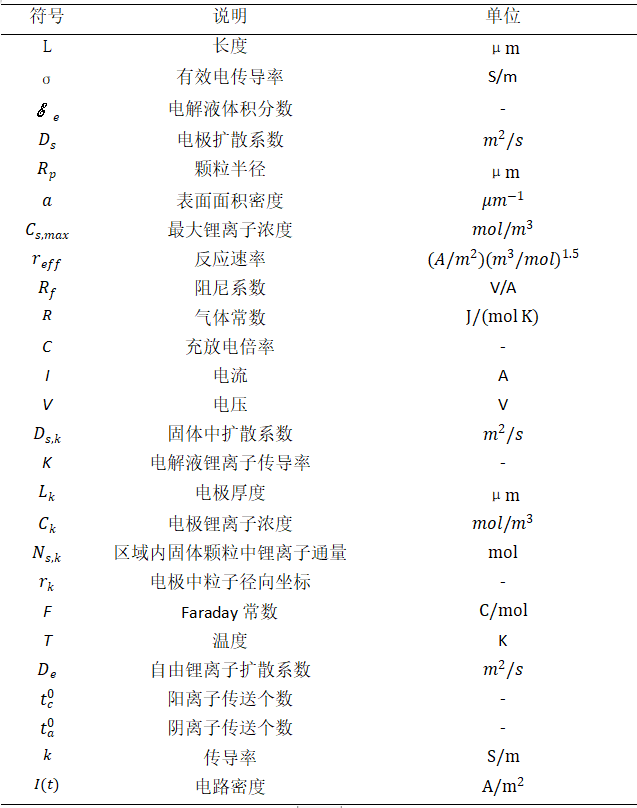
\includegraphics[scale = 0.7]{7}
\end{figure}




\section{模型的建立与求解}
\subsection{1单颗粒模型}
单颗粒模型是最简单的锂离子电池电化学模型,它是由传统$P2-D$模型\cite{Doyle1993Modeling}通过简化得来的。单颗粒模型是一种描述电池热力学、锂在电极活性物质中的扩散以及锂在电极/电解质界面插入/拔出反应的界面动力学的电化学电池模型。单颗粒模型采用两个球形颗粒分别表示锂离子电池的正极和负极,假设锂离子的嵌入脱出过程发生在球颗粒上,且认为电解液的浓度及其内部电势恒定不变。单颗粒模型结构简单,计算量小,所以容易实现在线应用。单粒子模型指的是利用一个球状粒子来代表整个电极而建立的一种电池简化数学模型,其简化为如下图\ref{a}所示。单颗粒模型整体是由两个球对称扩散方程组成:一个是典型的负粒子,另一个是典型的正粒子。在粒子的中心施加标准的无通量条件。由于单颗粒模型假设电极中所有粒子的行为都完全相同,粒子表面的通量就是电流除以电极的厚度。

\begin{figure}[h]
	\centering
	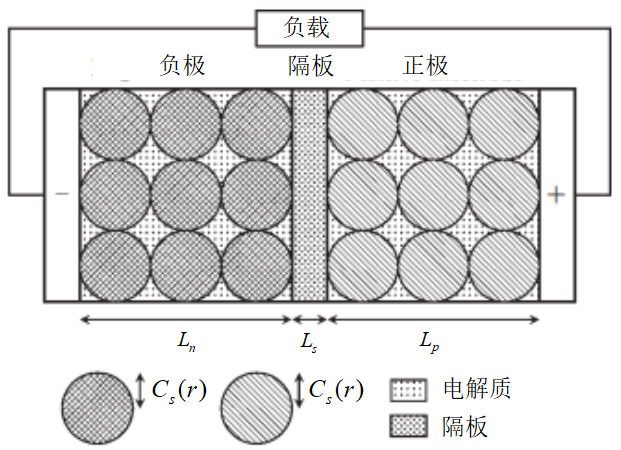
\includegraphics[scale = 0.4]{1}
	\caption{单颗粒模型}
	\label{a}
\end{figure}

作为单颗粒模型\cite{yuan2001determination},有优点也有缺点。其中多孔电极模型提供了对各种物理过程的复杂描述,拟合发生在电池中的各种物理过程,故该多孔电极模型在模拟时是非常耗时的。简化的单颗粒模型却能够极快地进行模拟,因为它并不监视所有的物理过程。比如模型建立忽略了固相扩散的限制,忽略了液相扩散过程,从而限制了模型的有效性。在模拟锂离子电池多个循环的性能时,需要在每个循环中反复求解电池模型。 理想情况下,模型在进行模拟时不消耗时间,并且还能提供在循环过程中发生的物理过程的真实描述。

目前,单颗粒模型主要应用于电池的荷电状态诊断研究(荷电状态SOC)。但同时锂离子电池单颗粒模型存在一些不可避免的缺点,即在大倍率充放电的条件下,模型的假设不合理,因此会不可避免的导致仿真偏差过大。

基于模型假设中的假设条件可知一个电极内各处的反应离子流密度也相等,这样电极内一个活性粒子的电化学特性就可以代表整个电极的特性\cite{santhanagopalan2006review},进而得到了电池的单粒子模型。由于电池内各处的液相溶度是均是相等的,因此可以忽略液相电势对电池端电压的影响。

每个电极的活性粒子总表面积$S_{i}$,可以根据活性材料的质量$w_i$,,活性材料的密度$\rho_{i}$和该电极活性粒子的半径$R_i$求解得到,其满足的关系表达式如下。
$$S_{i}=\frac{3}{R_{i}} \frac{w_{i}}{\rho_{i}}, \qquad i=p, n$$

接下来,根据电池的充放电电流值𝑰和电极的活性表面积𝑺𝒊进而求解得到每个电极内的反应离子流密度,即(F 为法拉第常数)
$$j_{i}=\frac{I}{F \cdot S_{i}}, \qquad i=p, n$$

正、负电极活性离子内的固相扩散过程满足 Fick 第二扩散定律,利用三参数抛物线近似方程来简化固相扩散过程,进而求解得到固相粒子表面的浓度。

具体求解过程如下,首先计算正、负极的体积平均浓度流量$\bar{q_i}(t)$,其关系表达式满足:
$$\frac{d}{d t} \bar{q}_{i}(t)+30 \frac{D_{s, i}}{R_{i}^{2}} \bar{q}_{i}(t)+\frac{45}{2} \frac{j_{i}}{R_{i}^{2}}=0, \qquad i=p, n$$

之后求解固相粒子内的锂离子平均浓度,其关系表达式满足:
$$\frac{d}{d t} \bar{c}_{s, i}(t)+3 \frac{j_{i}}{R_{i}}=0, i=p, n$$

其中,正、负极粒子内平均浓度的初始值分别为在大多数实际情况下是无法得到的准确值。所以通常把这两个参数看成待辨识的参数,最后,利用体积平均浓度流量和固相粒子内的平均浓度可以求解粒子表面的锂离子溶度,其表达式为:
$$c_{s, i}^{s u r f}(t)=\bar{c}_{s, i}(t)+\frac{R_{i}}{35 D_{s, i}}\left(8 D_{s, i} \bar{q}_{i}(t)-j_{i}\right)$$

为计算的简便性,引入正、负极的荷电状态电量,即为
$$\theta_{i}=\frac{C_{s, i}^{s u r f}(t)}{c_{s, i, \max }}$$
其中,$c_{s,i,\max}$为电极i活性粒子内的最大锂离子溶度。

通过实验进行模拟可以得到不同时刻正、负极的荷电状态变量值。在利用荷电状态与开路电势之间的关系表达式,就可以计算得到不同电荷状态下的开路电势$\phi_p$和$\phi_n$。

$j_i$是活性粒子单位面积上的电化学反应离子流密度,由Butler-Volmer方程可计算得到活性粒子表面的过电势值,该方程关系表达式满足:
$$j_{i}=2 k_{i} c_{s, i, \max }\left(1-\theta_{i}\right)^{0.5}\left(\theta_{i}\right)^{0.5} c^{0.5} \sinh \left(\frac{0.5 F}{R T} \eta_{i}\right),\qquad i=p, n$$
其中,$k_i$是电极i的电化学反应率常数,$\eta_{i}$为电势i的过电势,根据方程求解得到过电势的解为:
$$\eta_{i}=\frac{2 R T}{F} \ln \left(\frac{m_{i}+\sqrt{m_{i}^{2}+4}}{2}\right)$$

单粒子模型忽略了与液相扩散相关的反应过程,因此在电极中各个位置处的液相电势均为零,得到过电势与固相电势、开路电势满足的关系式为:
$$\eta_{i}=\Phi_{1, i}-U_{i}, i=p, n$$
其中,$\Phi_{1, i}$为电极i的固相电势,$U_{i}$为电极i的开路电势。

根据电池的内部物理特性可知:正极固相电势与负极固相电势之间的差值即为电池两端端电压(终端电压),表示为
$$V_{c e l l}=\Phi_{1, p}-\Phi_{1, n}=\left(U_{p}-U_{n}\right)+\left(\eta_{p}-\eta_{n}\right)$$

\subsection{2 Doyle-Fuller Newman(DFN)模型}
在多孔电极理论及浓溶液理论的基础上,通过考虑电池中各个物理化学反应原理如质量平衡,反应动力学和热动力学,Doyle等人在做出下列假设条件的基础下建立了锂离子电池的DFN模型\cite{Srinivasan_2002}\cite{BOTTE20002595}(如图\ref{b})。

\begin{figure}[h]
	\centering
	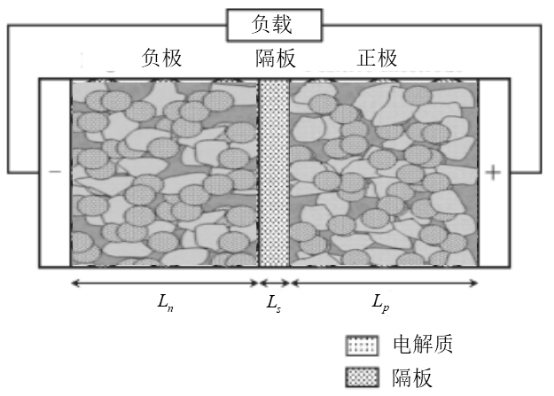
\includegraphics[scale = 0.5]{2}
	\caption{DFN模型}
	\label{b}
\end{figure}

根据锂离子电池的充放电过程,建立电池的准二维数学模型方程(DFN 模型方程)。DFN包括固体内部,固体和电解质中的电荷和质量守恒方程,还规定了在固体和电解质之间的界面上发生的电化学反应的行为。

根据第三章模型假设的条件,描述锂离子电池中的物理化学反应方程[4-7]有

1、bulter-volume方程:描述正、负极区域活性物质粒子内部的锂离子扩散过程。

2、固相扩散过程:描述正、负极区域活性物质粒子内部的锂离子扩散过程;

3、液相扩散过程:描述正、负极及隔膜区域内电解液中的锂离子扩散过程;

4、固相欧姆定律:描述正、负极区域内活性物质粒子的电势分布;

5、液相欧姆定律:描述正、负极及隔膜区域内液相电势的分布;

这样,就可以得到预测电池充放电行为的控制方程、初始条件以及边界条件。下面对锂离子电池内正极、隔膜和负极三个区域的模型方程进行描述。

\noindent\textbf{正极区域方程}

电池开始工作时,在电极球形粒子的表面上发生电化学反应,根据电池的工作电流,即可计算得到各处粒子表面上的反应离子流浓度。由 Butler-Volmer动力学方程可知,粒子表面的反应离子流浓度$j_p$与其表面上的过电势$\eta_{p}$满足关系表达式:
$$j_p = 2k_p(c_{s,p,max} - c_sI_{r=R_p})^{0.5}c_s|^{0.5}_{r=R_p}c^{0.5}sinh[\frac{0.5F}{RT}(\Phi_1-\Phi_2-U_p)]$$

其中$\Phi_1-\Phi_2-U_p = \eta_{p}$,$\eta_{p}$为正极过电势。在粒子表面发生电化学反应导致粒子表面的锂离子浓度发生变化,进而促进了球形粒子内的锂离子扩散,粒子内各处的锂离子浓度得到重新分布。

将正极的活性材料均看成是半径为$R_p$的球状粒子,则活性粒子内的锂离子浓度分布可根据 Fick 第二扩散定律求解得到:
$$\frac{\partial c_s}{\partial t} = \frac{D_{s,p}}{r^2}\frac{\partial}{\partial r}(r^2\frac{\partial c_s}{\partial r})$$

球形粒子内各处的锂离子初始浓度均相等,为$c_s|_{t=0} = c_{s,p,0}$

在粒子球心处的锂离子浓度流量始终为零,则有$\frac{\partial c_s}{\partial r}|_{r=0} = 0$

正极活性粒子表面处锂离子浓度的梯度和固相扩散率决定了粒子表面处的反应离子流浓度,得出粒子球面处的边界条件为
$$D_{s,p}\frac{\partial c_s}{\partial r}|_{r=R_p} = -j_p$$

由于球形粒子内发生固相扩散过程会导致该处电解液中的锂离子浓度发生变化,这样,在电极的电解液中由于锂离子浓度分布不均匀进而导致在电解液中发生锂离子扩散和迁移,电解液中的锂离子扩散方程\cite{Diwakar2009TowardsEM}满足:
$$\xi_p\frac{\partial c}{\partial t}=D_{eff,p}\frac{\partial^2 c}{\partial x^2}+\alpha_p(1-t_+)j_p$$

在电池工作的初始时刻,正极区域内各处液相浓度的均是一个常量,则在电极的任意位置处有$c|_{t=0} = c_0$

在正极集流体处由于没有液相锂离子沿着外电路的扩散或迁移,可知在该处的液相浓度流为 0,即$-D_{eff,p}\frac{\partial c}{\partial x}|_{x=0} = 0$

在正极与隔膜临界面出满足液相浓度流量连续,则有:
$$-D_{eff,p}\frac{\partial c}{\partial x}|_{x=r^-_p} = -D_{eff,p}\frac{\partial c}{\partial x}|_{x=i^*_p}$$

接下来根据固相欧姆定律得到正极区域的固相电势控制方程,该方程描述了正极区域内活性物质粒子电势的分布情况,即$i_1 = -\sigma_{eff,p}\frac{\partial \Phi_1}{\partial x}$。其中$i_1$为电池的固相电流(即电子电流),$\sigma_{eff,p}$为固相电导。

结合电池的工作原理可知,在正极集流体处仅有固相电流,即该处的固相电流等于电池的充放电电流,则在正极集流体处应满足的边界条件为:
$$\frac{\partial \Phi_1}{\partial x}|_{x=0} = -\frac{I}{\sigma_{eff,p}}$$
其中,$I$为电池的充放电电流(由总的放电电流除以电极面积得到)。充电时电流$I$为正数,放电时$I$为负数。

在隔膜区域不含有活性粒子,因此在该区域中没有电子的扩散或迁移过程,在隔膜区域不含有电子电流,仅有离子电流,且离子电流等于电池的充放电电流,因此在正极与隔膜临界面处满足的边界条件是电子电流为零,即
$$\frac{\partial \Phi_1}{\partial x}|_{x=l_p^-} = 0$$

电极中除了电子电流,另一个重要电流就是离子电流,在正极区域中的离子电流满足液相欧姆定律,该控制方程描述了正极区域内的液相电势分布[4],即
$$i_2 = -K_{eff,p}\frac{\partial \Phi_2}{\partial x} + 2\frac{K_{eff,p}RT}{F}(1-t_+)\frac{\partial ln c}{\partial x}$$

其中$i_2$为离子电流,$K_{eff,p}$是液相电导,该方程增加了液相锂离子浓度梯度对离子电流产生的影响,其中第一部分是液相电势梯度对离子电流作用的结果,第三部分是液相锂离子浓度梯度对离子电流作用的结果。

正极集流体处的离子电流为零,即液相电势流为零,则有
$$\frac{\partial \Phi_2}{\partial x}|_{x=0} = 0$$

在正极和隔膜临界面上的液相电势流连续,则有
$$-K_{eff,p}\frac{\partial \Phi_2}{\partial x}|_{x=l^-_p} = -K_{eff,s}\frac{\partial \Phi_2}{\partial x}|_{x=l^+_p}$$

根据电池内的物理化学反应过程,得出在电极中的任意位置处都有固相电子电流和液相离子电流之和等于电池总的充放电电流,即
$$i_1+i_2=I$$

同时还得到电子电流和离子电流梯度与该位置处的反应离子流密度$j_p$满足的关系表达式为
$$\frac{\partial i_1}{\partial x} = -a_pFj_p \qquad \qquad     \frac{\partial i_2}{\partial x} = a_pFj_p$$

综上所述,在正极区域有7个输出变量,它们是固相电势$\Phi_1$,液相电势$\Phi_2$,固相浓度$c_s$,液相浓度$c$,固相电子电流$i_1$,液相离子电流$i_2$以及正极反应离子流密度$j_p$\cite{Diwakar2009TowardsEM}。

\noindent\textbf{隔膜区域方程}

由于隔膜区域中不含有活性粒子,因此在该区域仅含有与液相有关的两个变量,液相浓度$c$和液相电势$\Phi_2$。同正极区域的液相锂离子扩散方程类似,建立隔膜区域的液相浓度扩散方程为
$$\xi_s\frac{\partial c}{\partial t} = D_{eff,s}\frac{\partial^2 c}{\partial x^2}$$

同样,在隔膜区域的初始液相浓度也为一个已知常量,则在该区域的任意位置处有$c|_{t=0} = c_0$。并且在隔膜与正、负极区域的临街面临满足液相锂离子浓度连续的条件,即
$$c|_{x=l_p^-}  = c|_{x=l_p^+} \qquad \qquad c|_{x=l_p+l_s^-}  = c|_{x=l_p+l_s^+}$$

由于隔膜区域不含有电子电流,所以隔膜区域各处的离子电流始终等于电池的充放电电流,则有
$$ -K_{eff,s}\frac{\partial \Phi_2}{\partial x} + 2\frac{K_{eff,s}RT}{F}(1-t_+)\frac{\partial lnc}{\partial x} = I$$

并且在隔膜与正、负极区域的临界面处满足液相电势连续的条件,即
$$\Phi_2|_{x=l_p^-}  = \Phi_2|_{x=l_p^+} \qquad \qquad \Phi_2|_{x=l_p+l_s^-}  = \Phi_2|_{x=l_p+l_s^+}$$

\noindent\textbf{负极区域方程}

同正极区域的模型方程类似,在负极区域有7个输出变量,它们是固相电势$\Phi_1$,液相电势$\Phi_2$,固相浓度$c_s$,液相浓度$c$,固相电子电流$i_1$,液相离子电流$i_2$以及正极反应离子流密度$j_p$\cite{Diwakar2009TowardsEM}。

首先根据Bulter-Volmer动力学方程建立了负极区域粒子表面的反应离子流浓度$j_p$与其表面上的过电势$\eta_{p}$满足关系表达式:
$$j_n = 2k_n(c_{s,n,max} - c_sI_{r=R_n})^{0.5}c_s|^{0.5}_{r=R_n}c^{0.5}sinh[\frac{0.5F}{RT}(\Phi_1-\Phi_2-U_n)]$$

其中$\Phi_1-\Phi_2-U_n = \eta_{n}$,$\eta_{n}$为V负极过电势。在粒子表面发生电化学反应导致粒子表面的锂离子浓度发生变化,进而促进了球形粒子内的锂离子扩散,粒子内各处的锂离子浓度得到重新分布。

将负极的活性材料均看成是半径为$R_p$的球状粒子,则活性粒子内的锂离子浓度分布可根据 Fick 第二扩散定律求解得到:
$$\frac{\partial c_s}{\partial t} = \frac{D_{s,n}}{r^2}\frac{\partial}{\partial r}(r^2\frac{\partial c_s}{\partial r})$$

负极活性粒子表面处锂离子浓度的梯度和固相扩散率决定了粒子表面处的反应离子流浓度,得出粒子球面处的初始条件和边界条件为
$$\frac{\partial c_s}{\partial r}|_{r=0} = 0 \qquad \qquad D_{s,n}\frac{\partial c_s}{\partial r}|_{r=R_n} = -j_n$$

在电池工作的初始时刻,正极区域内各处液相浓度的均是一个常量,则在电极的任意位置处有$c_s|_{t=0} = c_{n,0}$

由于球形粒子内发生固相扩散过程会导致该处电解液中的锂离子浓度发生变化,这样,在电极的电解液中由于锂离子浓度分布不均匀进而导致在电解液中发生锂离子扩散和迁移,负极区域电解液中的锂离子扩散和迁移过程满足的控制方程\cite{Diwakar2009TowardsEM}为:
$$\xi_n\frac{\partial c}{\partial t}=D_{eff,n}\frac{\partial^2 c}{\partial x^2}+\alpha_n(1-t_+)j_n$$


在负极与隔膜临界面出满足液相浓度流量连续,则有:
$$-D_{eff,s}\frac{\partial c}{\partial x}|_{x=l_p+l_s^-} = -D_{eff_n}\frac{\partial c}{\partial x}|_{x=l_p+l_s^+}$$

同正极集流体一样,负极集流体处不含有锂离子的扩散或迁移,因此该处的液相锂离子浓度流量始终为 0,即
$$-D_{eff_n}\frac{\partial c}{\partial x}|_{x=l_p+l_s+l_n} = 0$$

接下来根据固相欧姆定律得到正极区域的固相电势控制方程,该方程描述了正极区域内活性物质粒子电势的分布情况,即$i_1 = -\sigma_{eff,n}\frac{\partial \Phi_1}{\partial x}$。其中$i_1$为电池的固相电流(即电子电流),$\sigma_{eff,p}$为固相电导。

结合电池的工作过程可知,在隔膜区域不含有活性粒子,因此在该区域中没有电子的扩散或迁移过程,在隔膜区域不含有电子电流,仅有离子电流,且离子电流等于电池的充放电流,因此在负极与隔膜区域临界面处满足的边界条件是电子电流为零,即
$$\frac{\partial \Phi_2}{\partial x}|_{x=l_p+l_n^-} = 0$$

在负集流体处仅有电子电流,即该处的电子电流等于总的放电电流,则在负集流体处应该满足的边界条件为
$$\frac{\partial \Phi_1}{\partial x}|_{x=l_p+l_s+l_n} = -\frac{I}{\sigma_{eff,n}}$$
其中,$I$为电池的充放电电流(由总的放电电流除以电极面积得到)。充电时电流$I$为正数,放电时$I$为负数。

利用液相欧姆定律得到液相电势的控制方程为
$$i_2 = -K_{eff,n}\frac{\partial \Phi_2}{\partial x} + 2\frac{K_{eff,n}RT}{F}(1-t_+)\frac{\partial ln c}{\partial x}$$

同理可知,隔膜和负极区域临界面处的液相电势流连续,则有
$$-K_{eff,s}\frac{\partial \Phi_2}{\partial x}|_{x=l_p+l^-_s} = -K_{eff,n}\frac{\partial \Phi_2}{\partial x}|_{x=l_p+l^+_s}$$

在隔膜区域不含有活性粒子,因此在该区域中没有电子的扩散或迁移过程,在隔膜区域不含有电子电流,仅有离子电流,且离子电流等于电池的充放电电流,因此在正极与隔膜临界面处满足的边界条件是电子电流为零,即
$$\frac{\partial \Phi_1}{\partial x}|_{x=l_p^-} = 0$$

其中,把负极集流体处的液相电势定义为零来作为整个电池的一个参考电势,即
$$\Phi_2|_{x=l_p+l_s+l_n} = 0$$

根据电池内的物理化学反应过程,得出在电极中的任意位置处都有固相电子电流和液相离子电流之和等于电池总的充放电电流,即
$$i_1+i_2=I$$

同时还得到电子电流和离子电流梯度与该位置处的反应离子流密度$j_p$满足的关系表达式为
$$\frac{\partial i_1}{\partial x} = -a_nFj_n \qquad \qquad     \frac{\partial i_2}{\partial x} = a_nFj_n$$

\subsection{3单颗粒模型求解}
\noindent\textbf{单颗粒单组参数求解}

我们使用pybamm工具包\cite{Sulzer2021}对单颗粒取最初始的参数进行模拟研究。在时间维度统一的研究了单颗粒模型在电池进行放电操作时,模型中相关物理量对于时间的变化(如图\ref{c}所示)。特别说明的是Electrolyte concentration(电解质溶度)和Electrolyte potential(电解质电位)对于时间的变化相同的原因是我们研究的是两极板的中心点位置各个物理量对于时间的变化规律。
\begin{figure}[h]
	\centering
	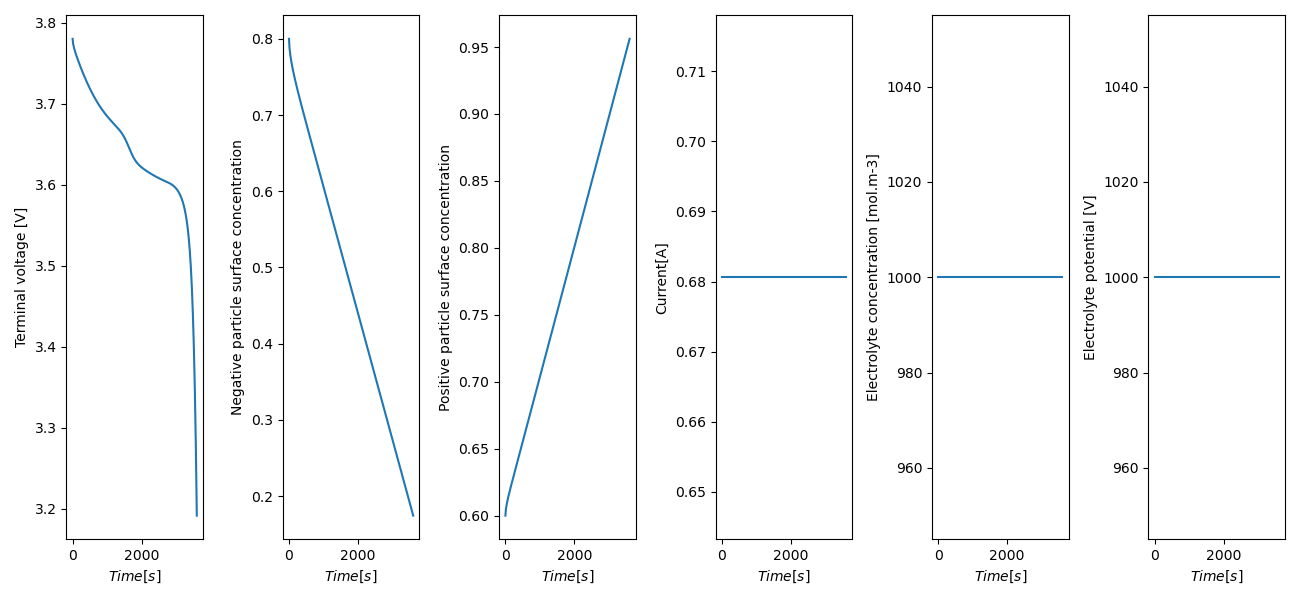
\includegraphics[scale = 0.4]{SPM}
	\caption{单颗粒模型模拟放电图}
	\label{c}
\end{figure}

Negative particle surface concentration(负粒子溶度):放电时,随着时间的变化,负粒子溶度下降,负电极中颗粒的锂离子扩散到颗粒表面,发生电化学反应残生锂离子和电子,自由锂离子通过电解质扩散到正极区,故粒子溶度一直下降。

Positive particle surface concentration(正粒子溶度):放电时,随着时间的变化,正粒子溶度上升,负电极中颗粒的锂离子扩散到颗粒表面,发生电化学反应残生锂离子和电子,自由锂离子通过电解质扩散到正极区,故正粒子溶度一直上升。

Electrolyte concentration(电解质溶度):因为使用的SPM模型进行测试,SPM模型中假设电解质溶度不变,故电解质溶度是不随时间变化。

Current(电流):因为SPM采用的恒定电流测试,故电流不会发生改变。

Electrolyte potential(电解质电位):单粒子模型认为内部电势恒定不变,电子从负极通过外部电路转到正极,负极电势相对内部电势降低,故电解质电位相当于负极电位降低。

Terminal voltage(电压):随着电子经外环路从负极到正极,正负极之间的电势差逐渐减少,电压也逐渐减小。

Negative electrode potential(负电极电位):该电位电势对地电势一直为0,不发生改变。

Positive electrolyte potential(正电极电位):随着单颗粒锂离子电池模型中电子从负电极电位转移到正电极电位转移,电子于正电极表面粒子发生中和反应。导致正电极表面粒子溶度降低,进而对地(负电极)电势降低,表现为正电极电位降低。

对于单颗粒模型的内部的空间进一步的进行了模拟研究,可以获得各个时间段对于空间中每个位置中的物理量进行模拟研究。可以得到以下结果图(如图\ref{d}图\ref{f}图\ref{g}所示)
\begin{figure}[h]
	\centering
	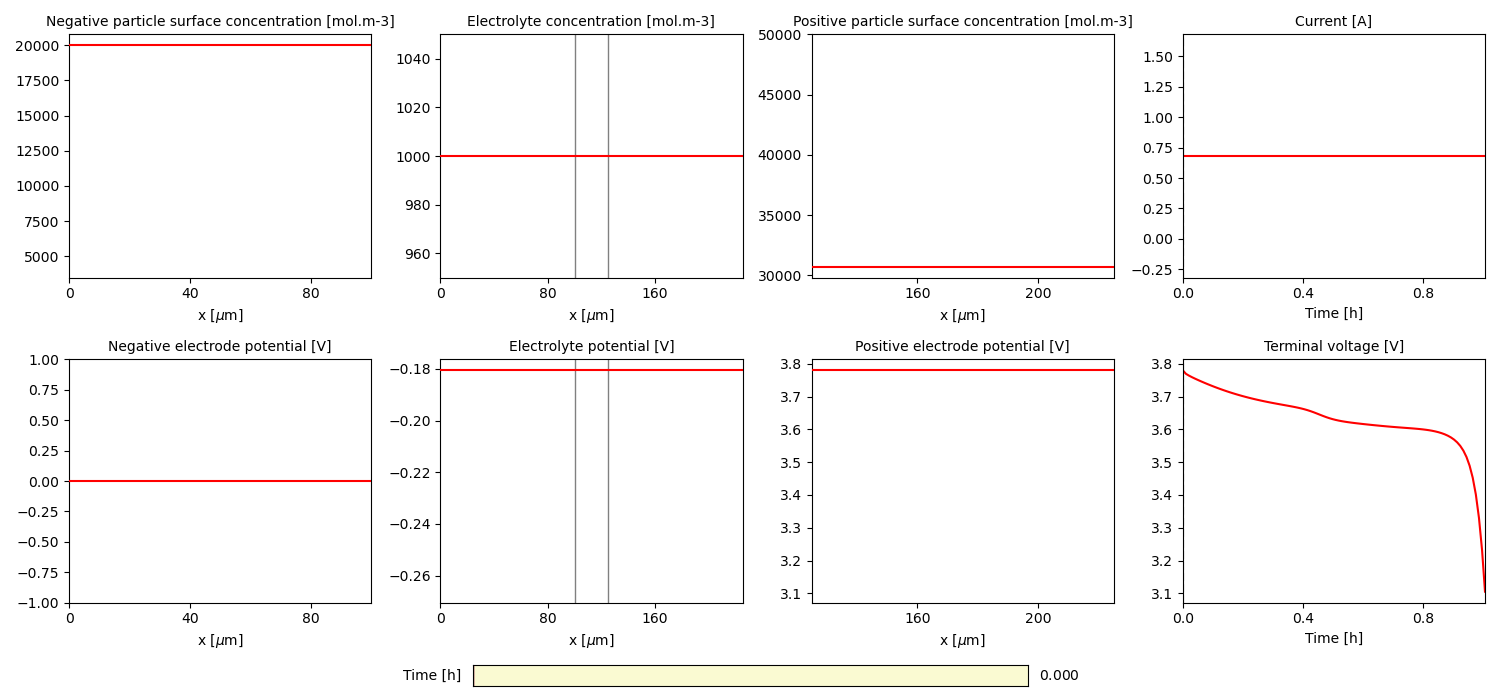
\includegraphics[scale = 0.4]{SPM0}
	\caption{单颗粒模型初始放电各位置物理量大小图}
	\label{d}
\end{figure}

\begin{figure}[H]
	\centering
	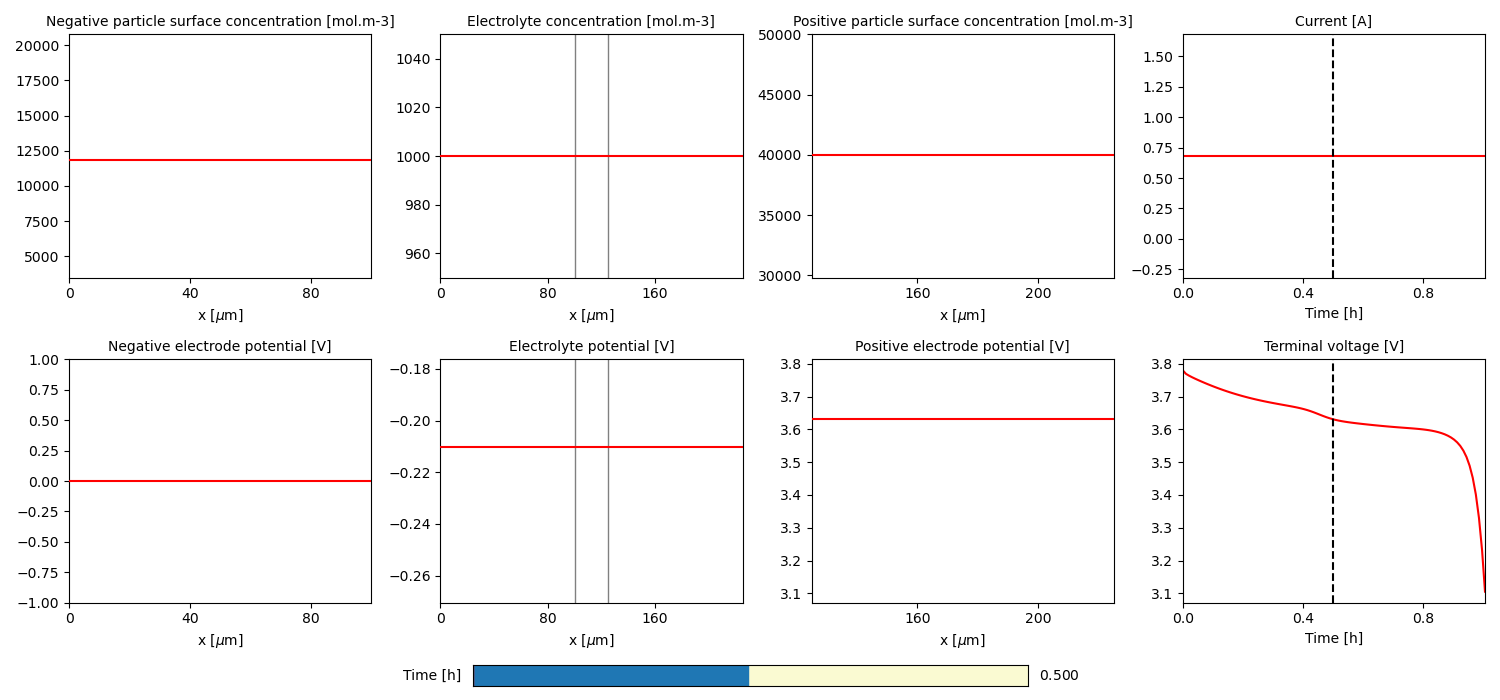
\includegraphics[scale = 0.4]{SPM2}
	\caption{单颗粒模型放电半小时各位置物理量大小图}
	\label{f}
\end{figure}

\begin{figure}[H]
	\centering
	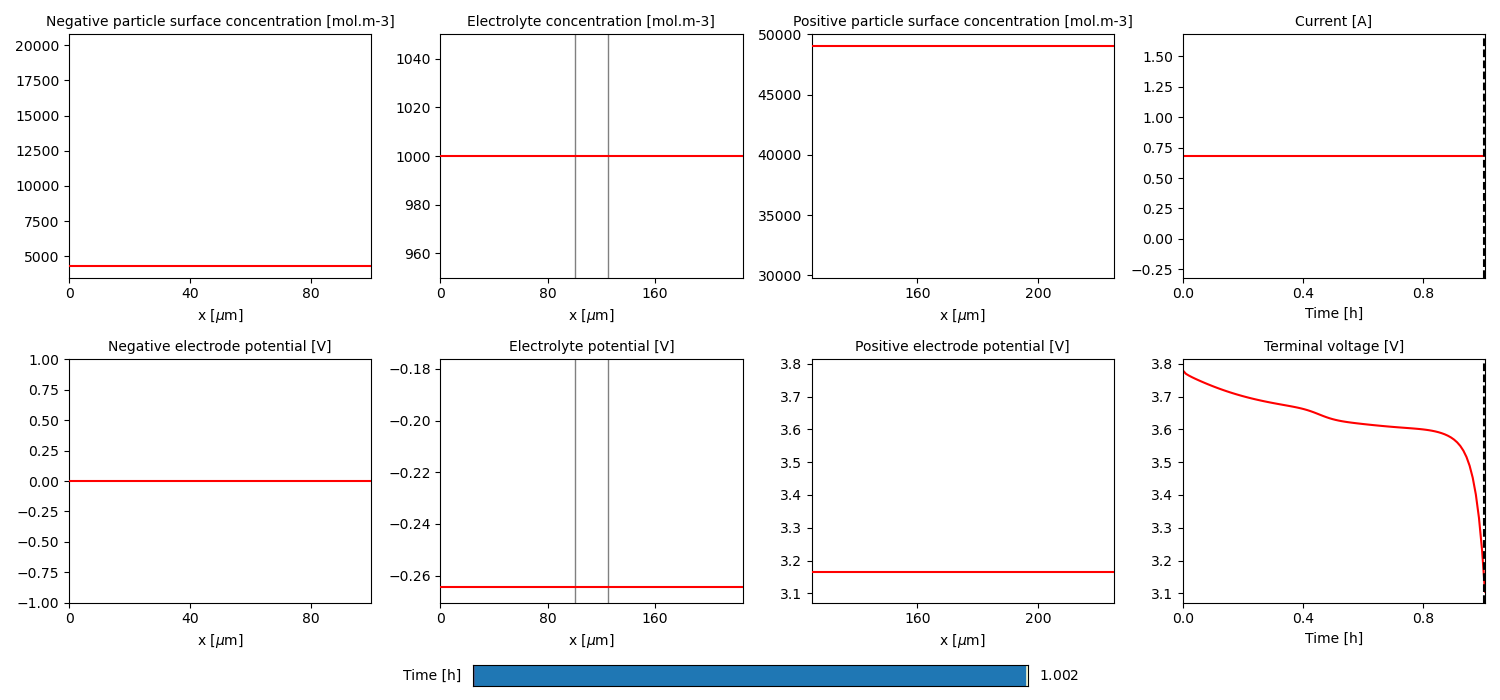
\includegraphics[scale = 0.4]{SPM1}
	\caption{单颗粒模型放电一小时各位置物理量大小图}
	\label{g}
\end{figure}

单粒子模型放电时:负极中处于栅格位置的锂离子发生化学反应释放自由锂离子,锂离子进入电解液中,运输到正极。在正极中,自由锂离子经过化学反应插入到正极的栅格位置,发生反应产生的电子通过电路从负极进入正极。充电时:正极中处于栅格位置的锂离子发生化学反应释放自由锂离子,锂离子进入电解液中,运输到负极。在负极中,自由锂离子经过化学反应插入到负极的栅格位置,发生反应产生的电子通过电路从正极进入负极。

\noindent\textbf{单颗粒多组参数求解}

在对单颗粒模型进行模拟操作时,提供了许多参数可以进行调节,以更为的切合于实际情况。本文主要讨论模型参数中较为重要的参数如温度,电极内颗粒内的扩散类型。

\noindent\textbf{1.温度对锂离子电池的影响:}

温度对电池的内阻、充电性能、放电性能、安全性、寿命等都会造成不同程度的影响。对于锂离子电池,低温条件下放电量会加剧,但在高温情况下放电量比常温低,主要是高温情况下锂离子迁移速度加快,锂电极和贮氢电极在高温情况下产生分解或形成氢气使电量消耗减少。而在低温环境下锂离子活动迟缓,需要更大的电压驱动电池进行正常工作,于是造成了电池更大的消耗。

对于锂电池来说,目前业内尚未有明确的理论支撑其各温度性能下的内阻、放电平台、寿命、容量等必然联系,相关的计算公式和数学模型还在摸索阶段。大体上,锂电池对0-40℃这个区间的温度并不敏感,然而一旦温度超过这个区间,寿命和容量就会打折扣。

参数:thermal(温度),有4种参数选择,“isothermal”(恒温),“lumped”(集中),“x-lumped(x-集中)”,“x-full(x-充满)”

Isothermal的结果图像和lumped的结果图像相同,电位电势和电压比其他两种情况下降更快 “x-lumped”,“x-full”两种情况下降缓慢,相对另外两种情况电池可以使用更长的时间。(如图\ref{h}图\ref{i}图\ref{j})

\begin{figure}[h]
	\centering
	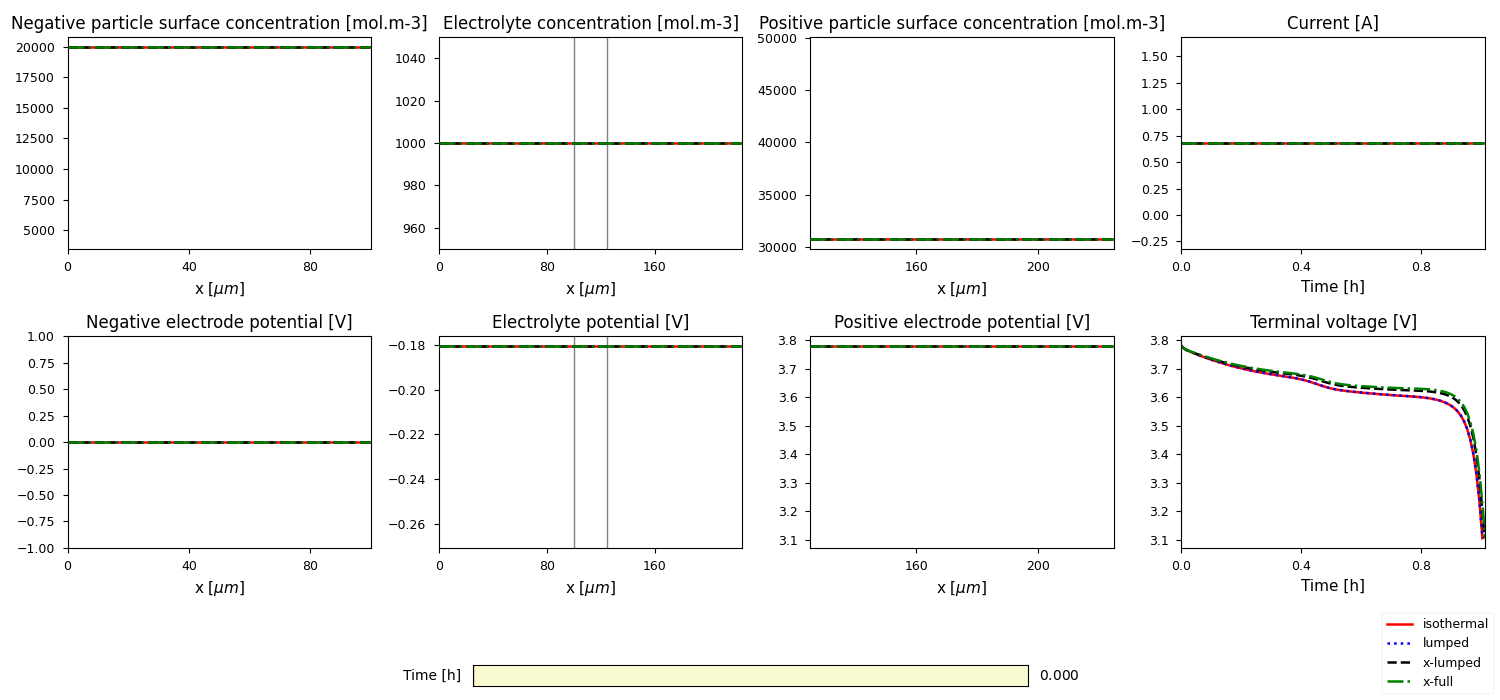
\includegraphics[scale = 0.4]{T0}
	\caption{单颗粒模型初始放电温度影响对比图}
	\label{h}
\end{figure}

\begin{figure}[H]
	\centering
	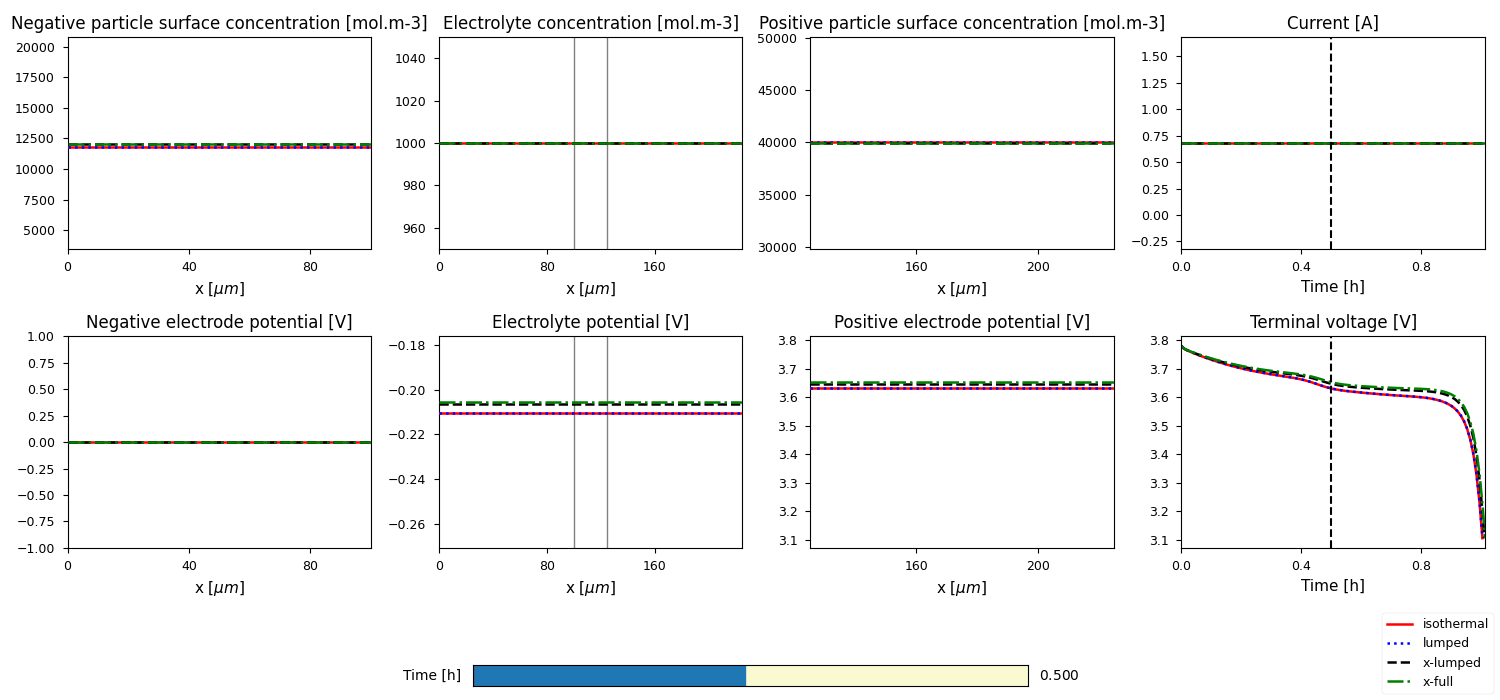
\includegraphics[scale = 0.4]{T1}
	\caption{单颗粒模型放电半小时温度影响对比图}
	\label{i}
\end{figure}

\begin{figure}[H]
	\centering
	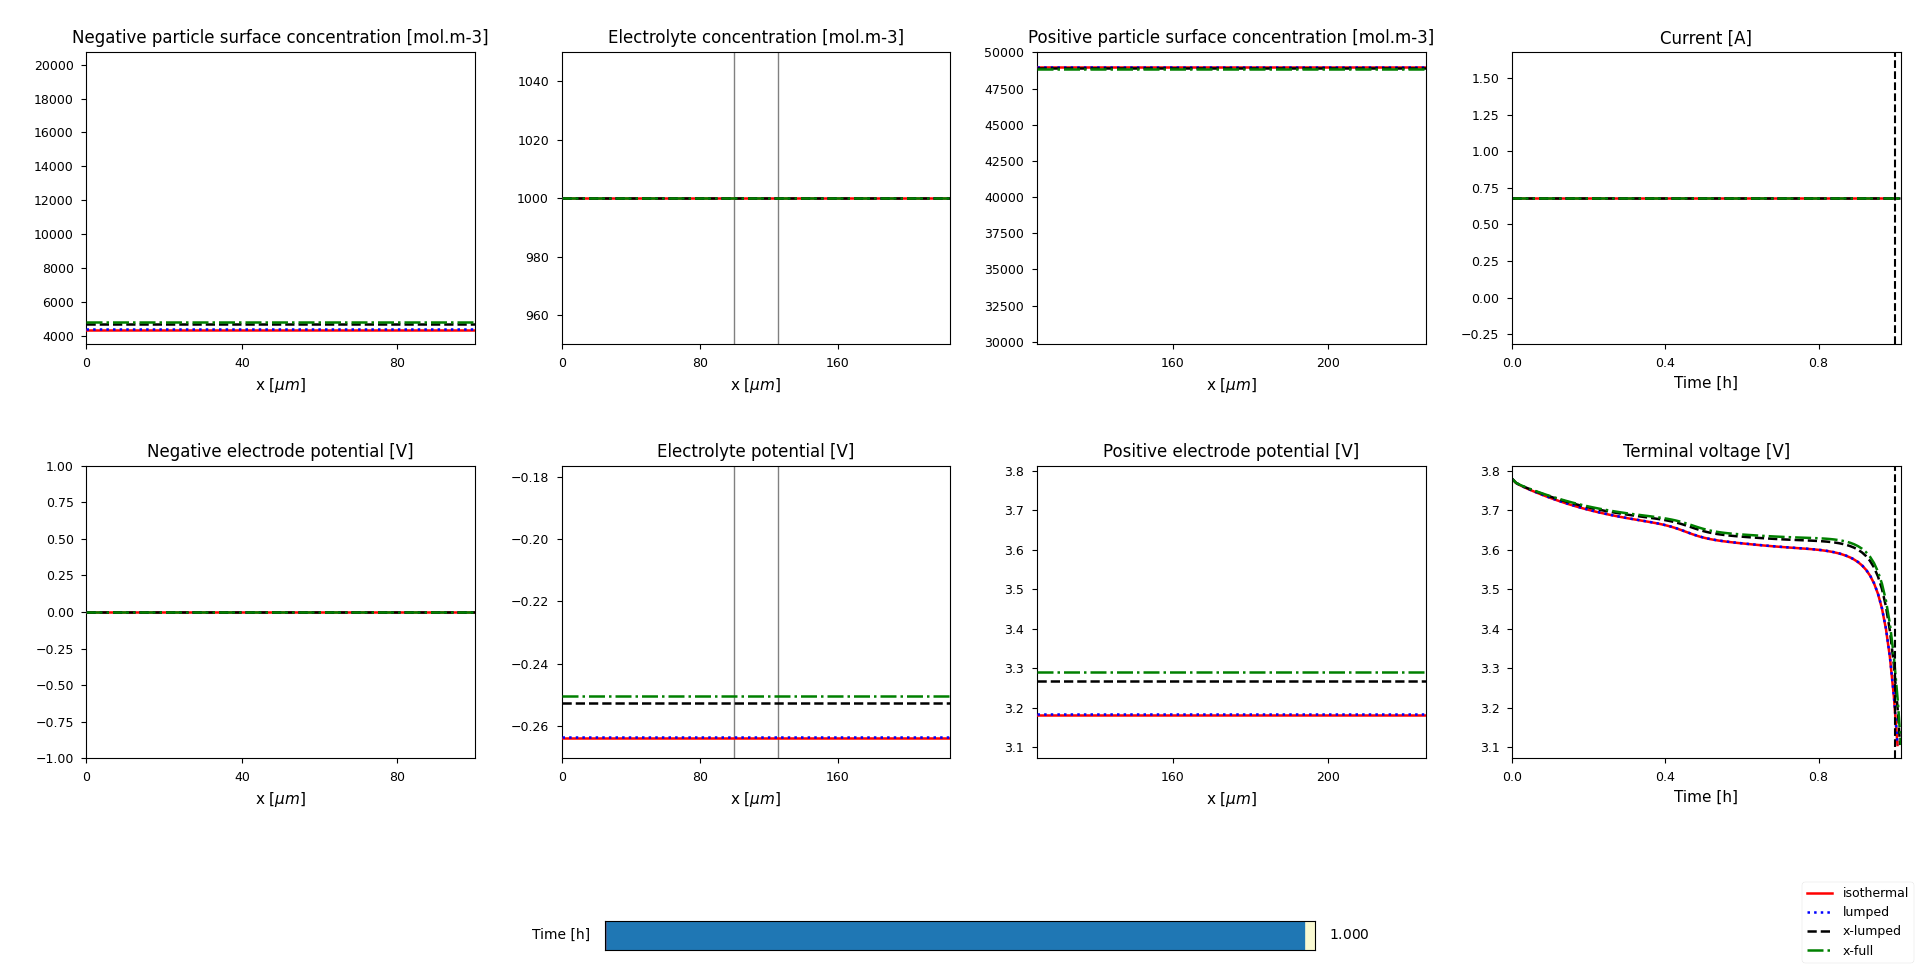
\includegraphics[scale = 0.32]{T2}
	\caption{单颗粒模型放电一小时温度影响对比图}
	\label{j}
\end{figure}

由于锂电池内部的化学反应与温度密切相关,因此锂电池组的热量消耗率在不同温度下会有所不同。环境温度低,并且锂电池组在运行期间会自行产生更多的热量。锂电池的工作环境温度对内阻,热耗率,放电容量,循环寿命和电池状态的一致性有一定的影响。我们在使用磷酸铁锂电池组的时候要尽量把工作环境控制在一个较好的温度环境之下。温度的异常会对锂离子电池的性能、寿命产生巨大影响,甚至可能发生热失控等安全问题,因此散热优秀的锂电池才是合格的锂电池。

另外我们对比了温度参数对单颗粒模型的充放电的过程的影响(如图\ref{aa})
\begin{figure}[h]
	\centering
	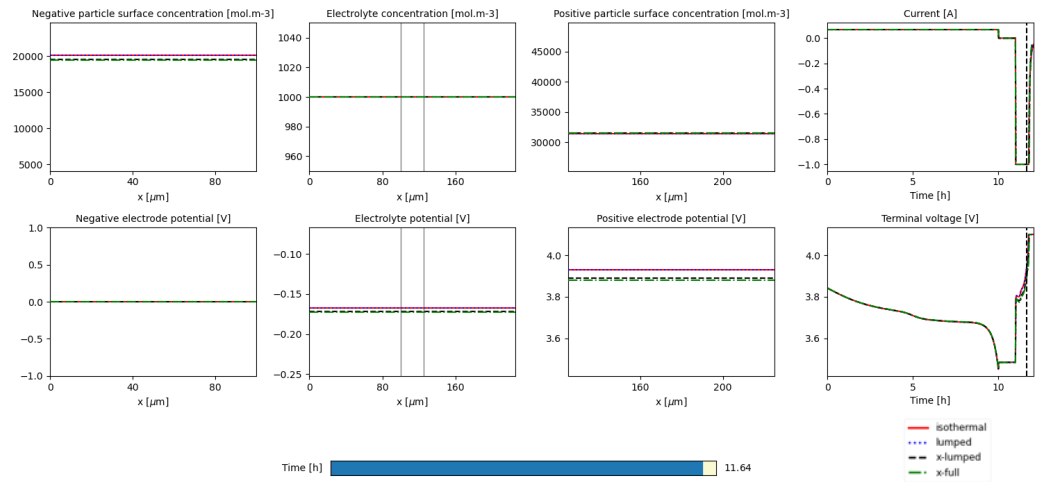
\includegraphics[scale = 0.4]{6}
	\caption{单颗粒模型充放电温度影响对比图}
	\label{aa}
\end{figure}

\noindent\textbf{2.电极内颗粒的扩散类型对锂离子电池的影响:}

溶液中离子的扩散是溶液的基本性质,是微粒(分子、原子)的热运动而产生的物质迁移现象,主要由浓差、温差和湍流运动引起,研究扩散可为溶液结构提供信息。扩散现象是指物质分子从高浓度区域向低浓度区域转移直到均匀分布的现象,速率与物质的浓度梯度成正比。扩散现象是一个基于分子热运动的输运现象,是分子通过布朗运动从高浓度区域(或高化势)向低浓度区域(或低化势)的运输的过程。它是趋向于热平衡态的驰豫过程,是熵驱动的过程。由于扩散作用的速率和混合物的浓度梯度一般不太大,因此通常可以用近平衡态热力学理论进行处理。扩散是由于分子热运动而产生的质量迁移现象,主要是由于密度差引起的。分子热运动认为在绝对零度不会发生。扩散现象等大量事实表明,一切物质的分子都在不停地做无规则的运动。

菲克第一定律只适应于J和C不随时间变化——稳态扩散(Steady-state diffusion)的场合。所谓稳定扩散是指扩散过程中扩散物质的浓度分布不随时间变化的扩散过程,这类问题可直接用菲克第一定律解决。对于稳态扩散也可以描述为:在扩散过程中,各处的扩散组元的浓度C只随距离x变化,而不随时间t变化,每一时刻从前边扩散来多少原子,就向后边扩散走多少原子,没有盈亏,所以浓度不随时间变化。

另外我们还采用了均匀分布扩散模型,二次分布扩散模型,四次分布扩散模型对于单粒子模型进行了模拟分析结果,具体结果如图\ref{l}图\ref{m}图\ref{n}。
\begin{figure}[h]
	\centering
	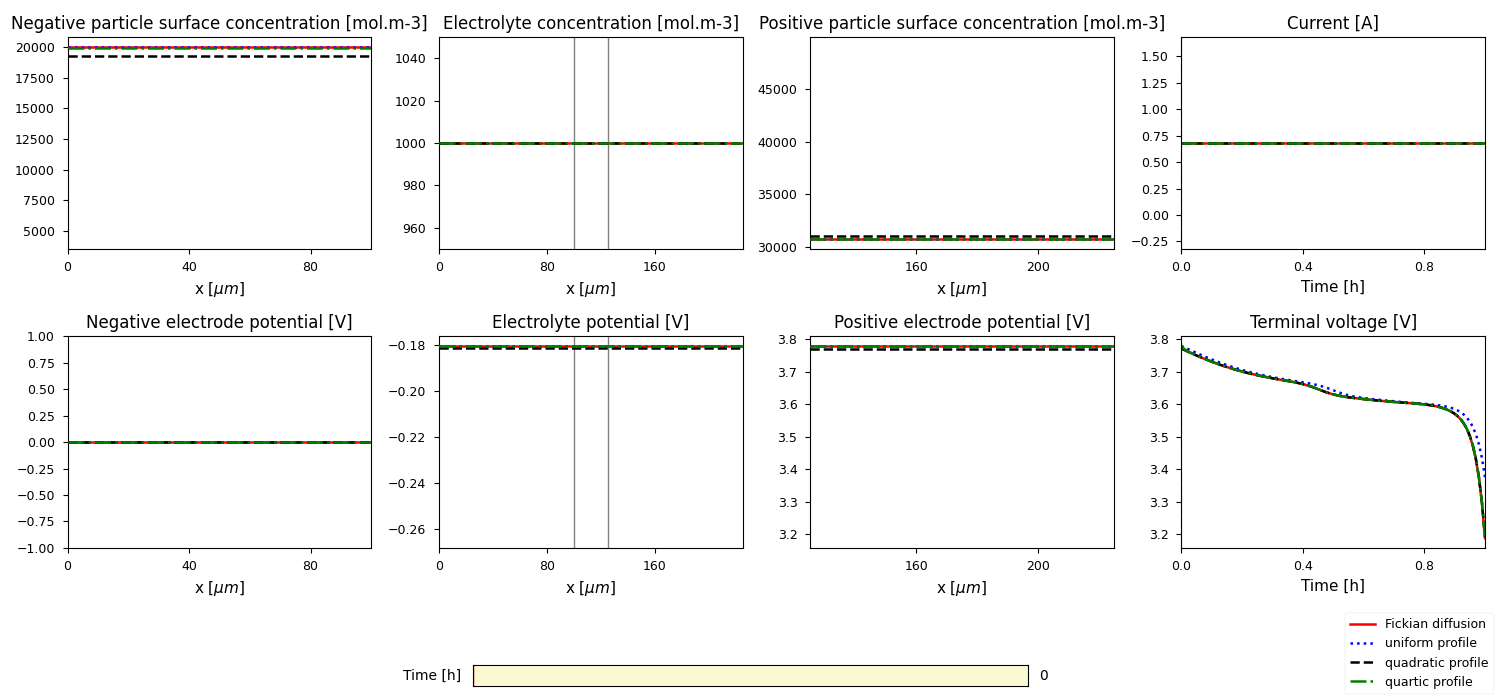
\includegraphics[scale = 0.4]{K0}
	\caption{单颗粒模型初始放电扩散类型影响对比图}
	\label{l}
\end{figure}

\begin{figure}[H]
	\centering
	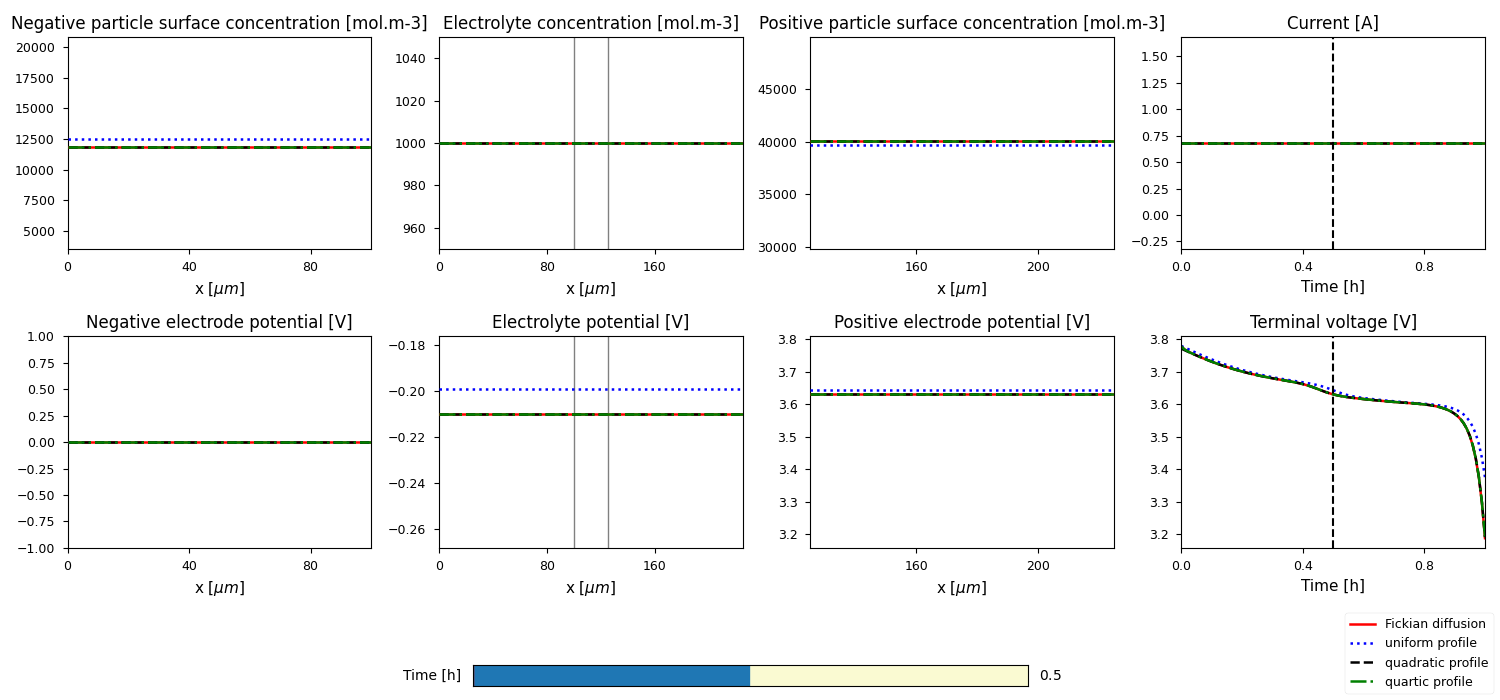
\includegraphics[scale = 0.4]{K1}
	\caption{单颗粒模型放电半小时扩散类型影响对比图}
	\label{m}
\end{figure}

\begin{figure}[H]
	\centering
	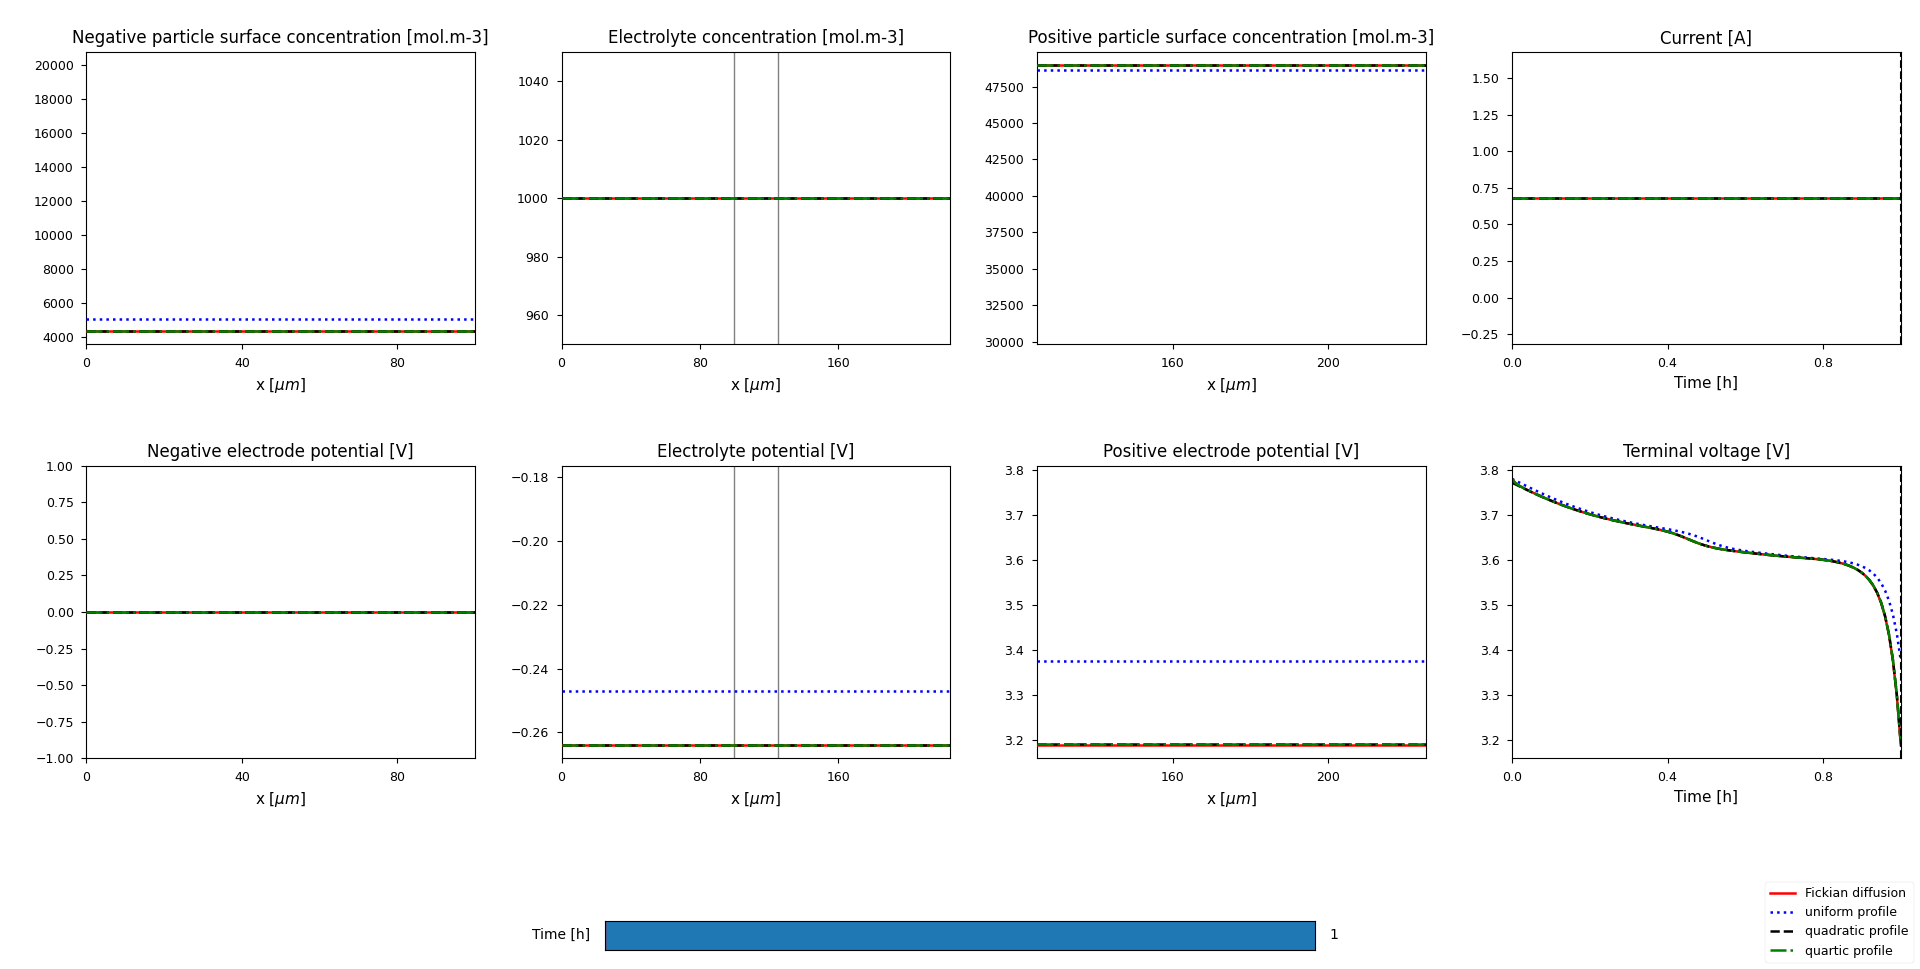
\includegraphics[scale = 0.32]{K2}
	\caption{单颗粒模型放电一小时扩散类型影响对比图}
	\label{n}
\end{figure}

实验结果表明,对于单颗粒模型的扩散二次分布扩散模型,四次分布扩散模型,菲克第一定律对于模型的模拟相差无几,而均匀分布扩散模型,随着扩散的程度加深,于其他扩散模型在粒子在空间中的分布有了明显的差别。

另外我们对比了温度参数对单颗粒模型的充放电的过程的影响(如图\ref{bb})
\begin{figure}[h]
	\centering
	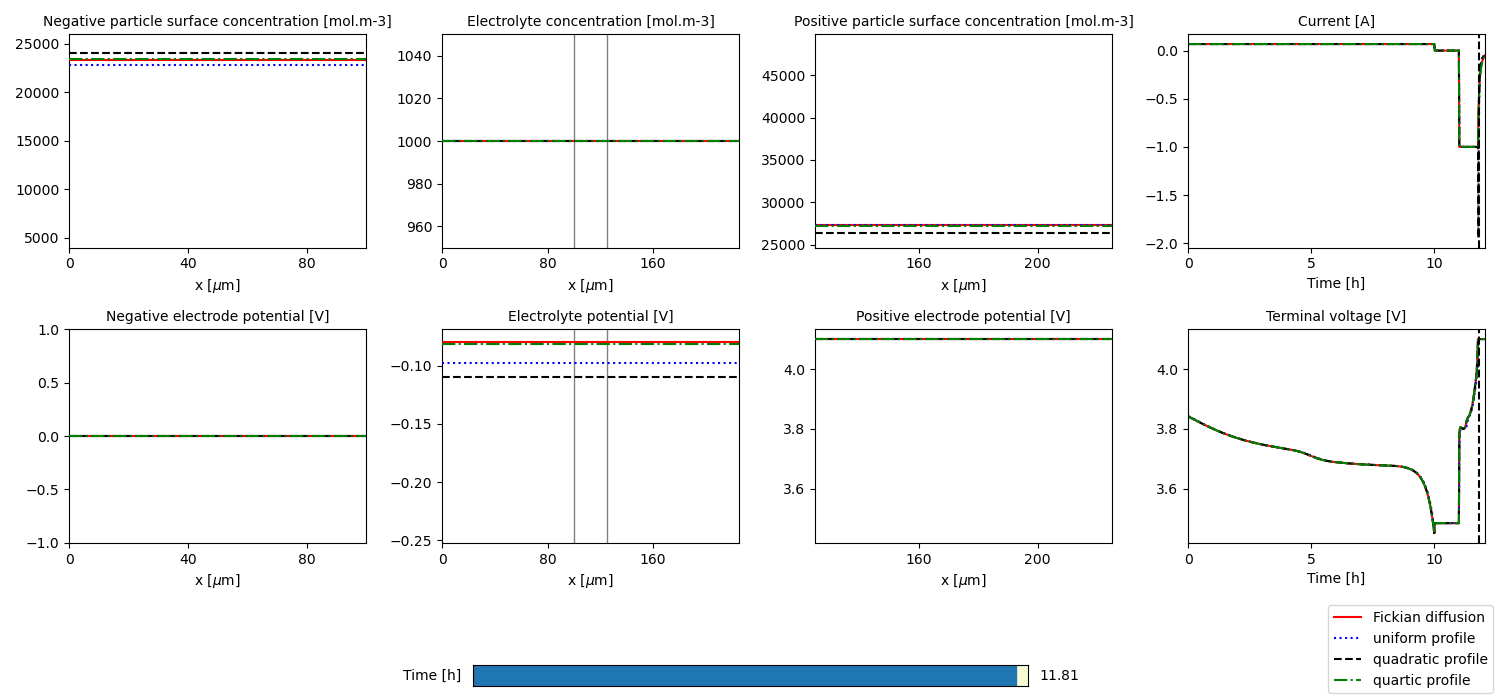
\includegraphics[scale = 0.4]{5}
	\caption{单颗粒模型充放电扩散类型影响对比图}
	\label{bb}
\end{figure}

\subsection{4Doyle-Fuller Newman(DFN)模型求解并对比}
我们使用pybamm工具包对DFN模型取最初始的参数进行模拟研究。在时间维度统一的研究了DFN模型在电池进行放电操作时,模型中相关物理量对于时间的变化,并对DFN模型和单颗粒模型进行比较(如图\ref{o}图\ref{p}图\ref{q}所示)。

\begin{figure}[h]
	\centering
	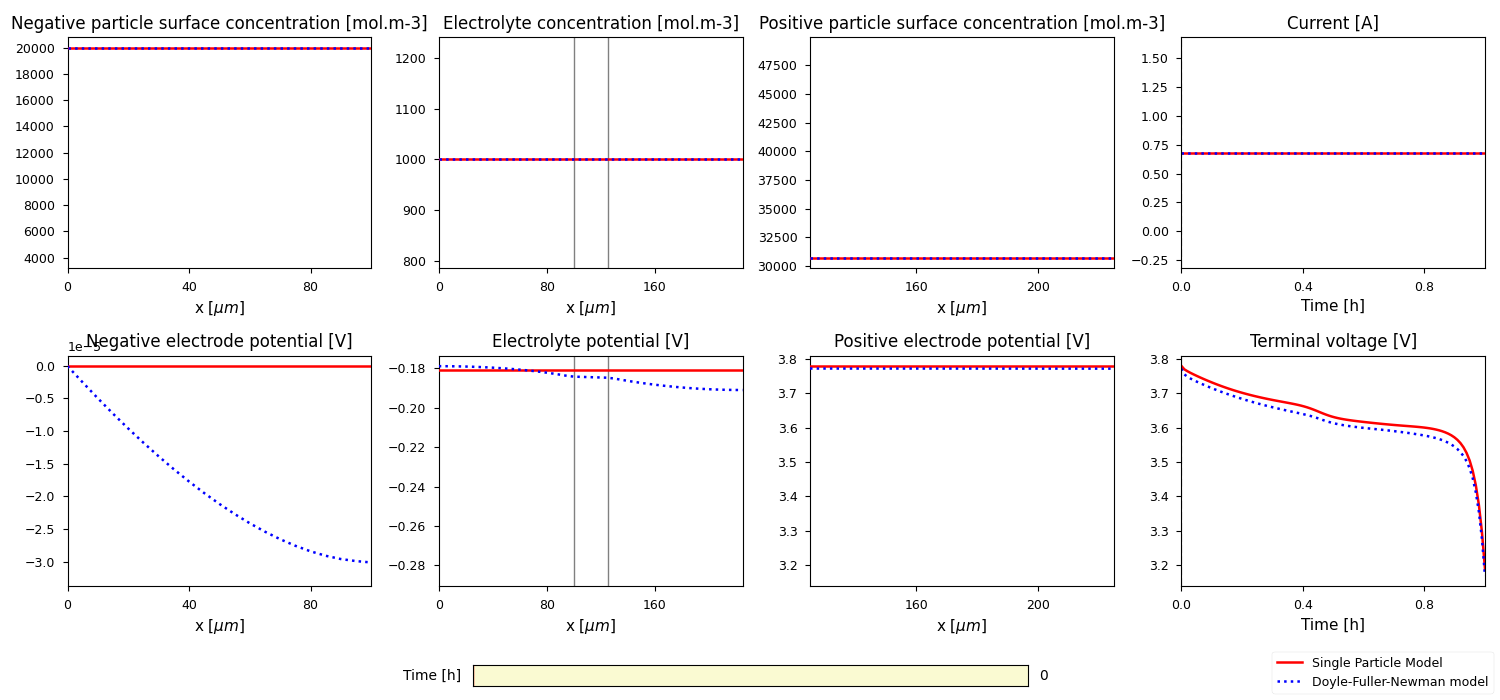
\includegraphics[scale = 0.4]{SPM-DFN1}
	\caption{单颗粒模型和DFN模型初始放电对比图}
	\label{o}
\end{figure}

\begin{figure}[H]
	\centering
	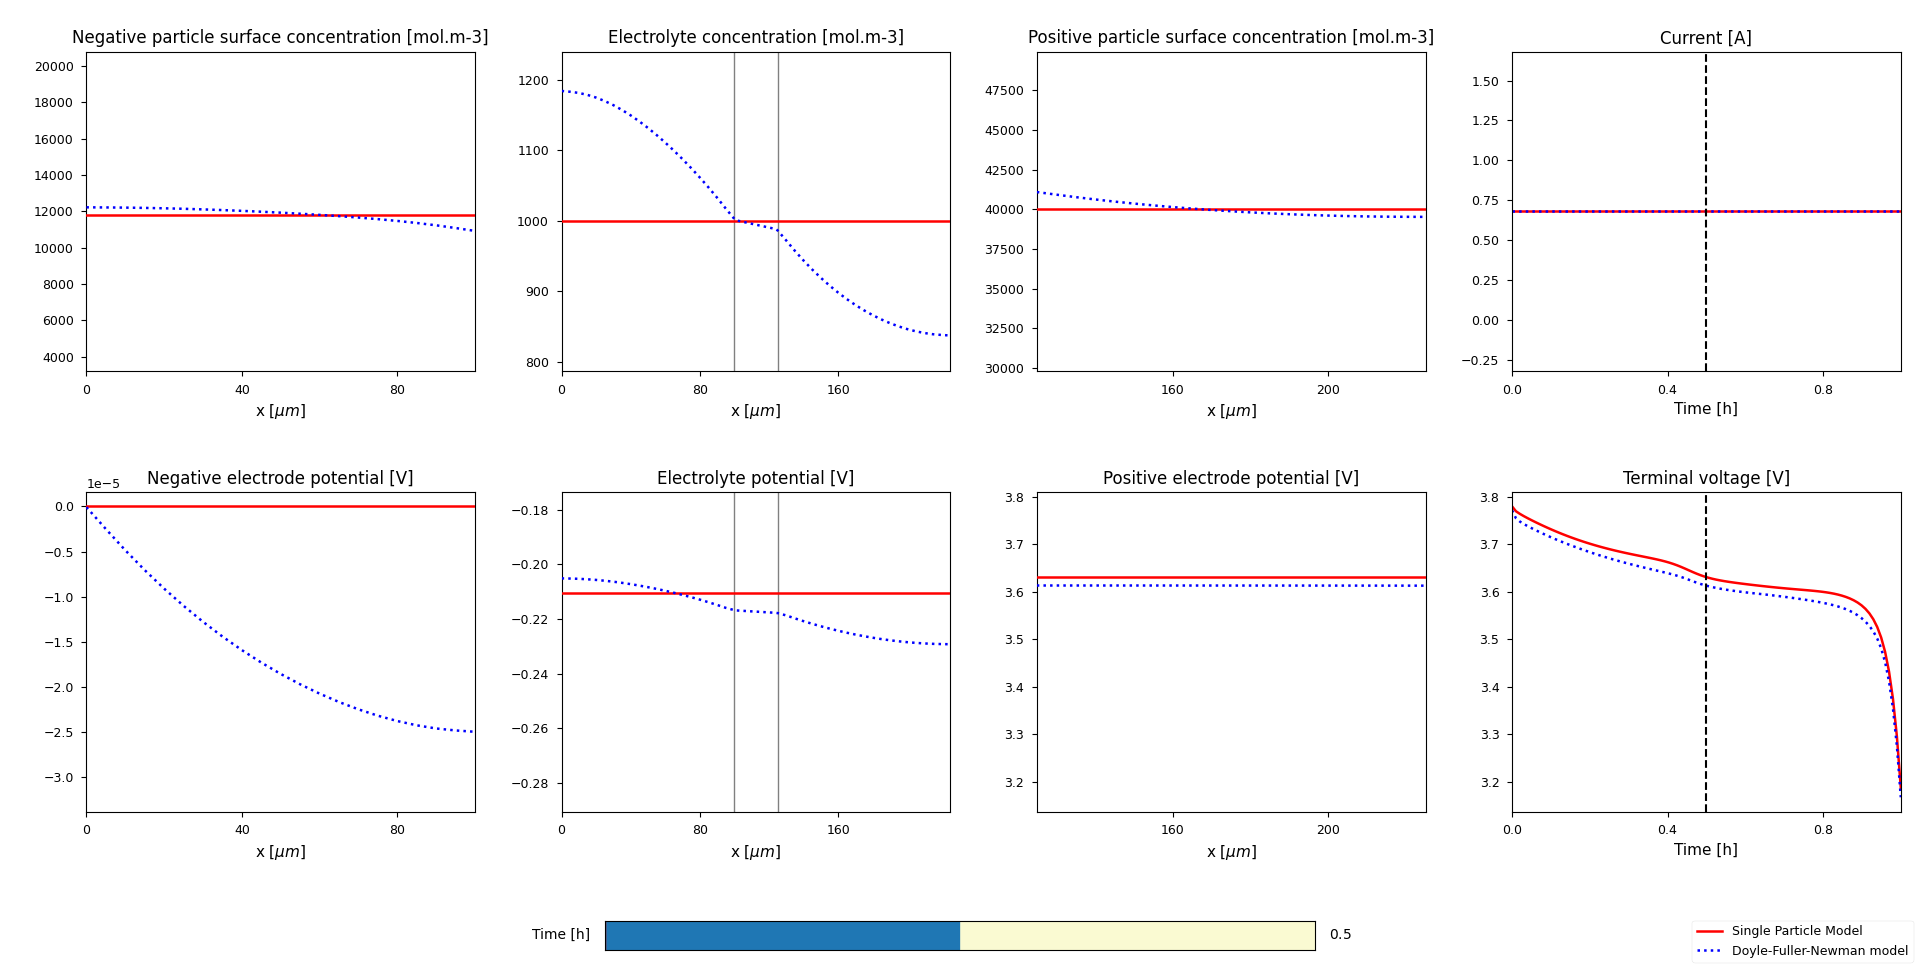
\includegraphics[scale = 0.32]{SPM-DFN2}
	\caption{单颗粒模型和DFN模型放电半小时对比图}
	\label{p}
\end{figure}

\begin{figure}[H]
	\centering
	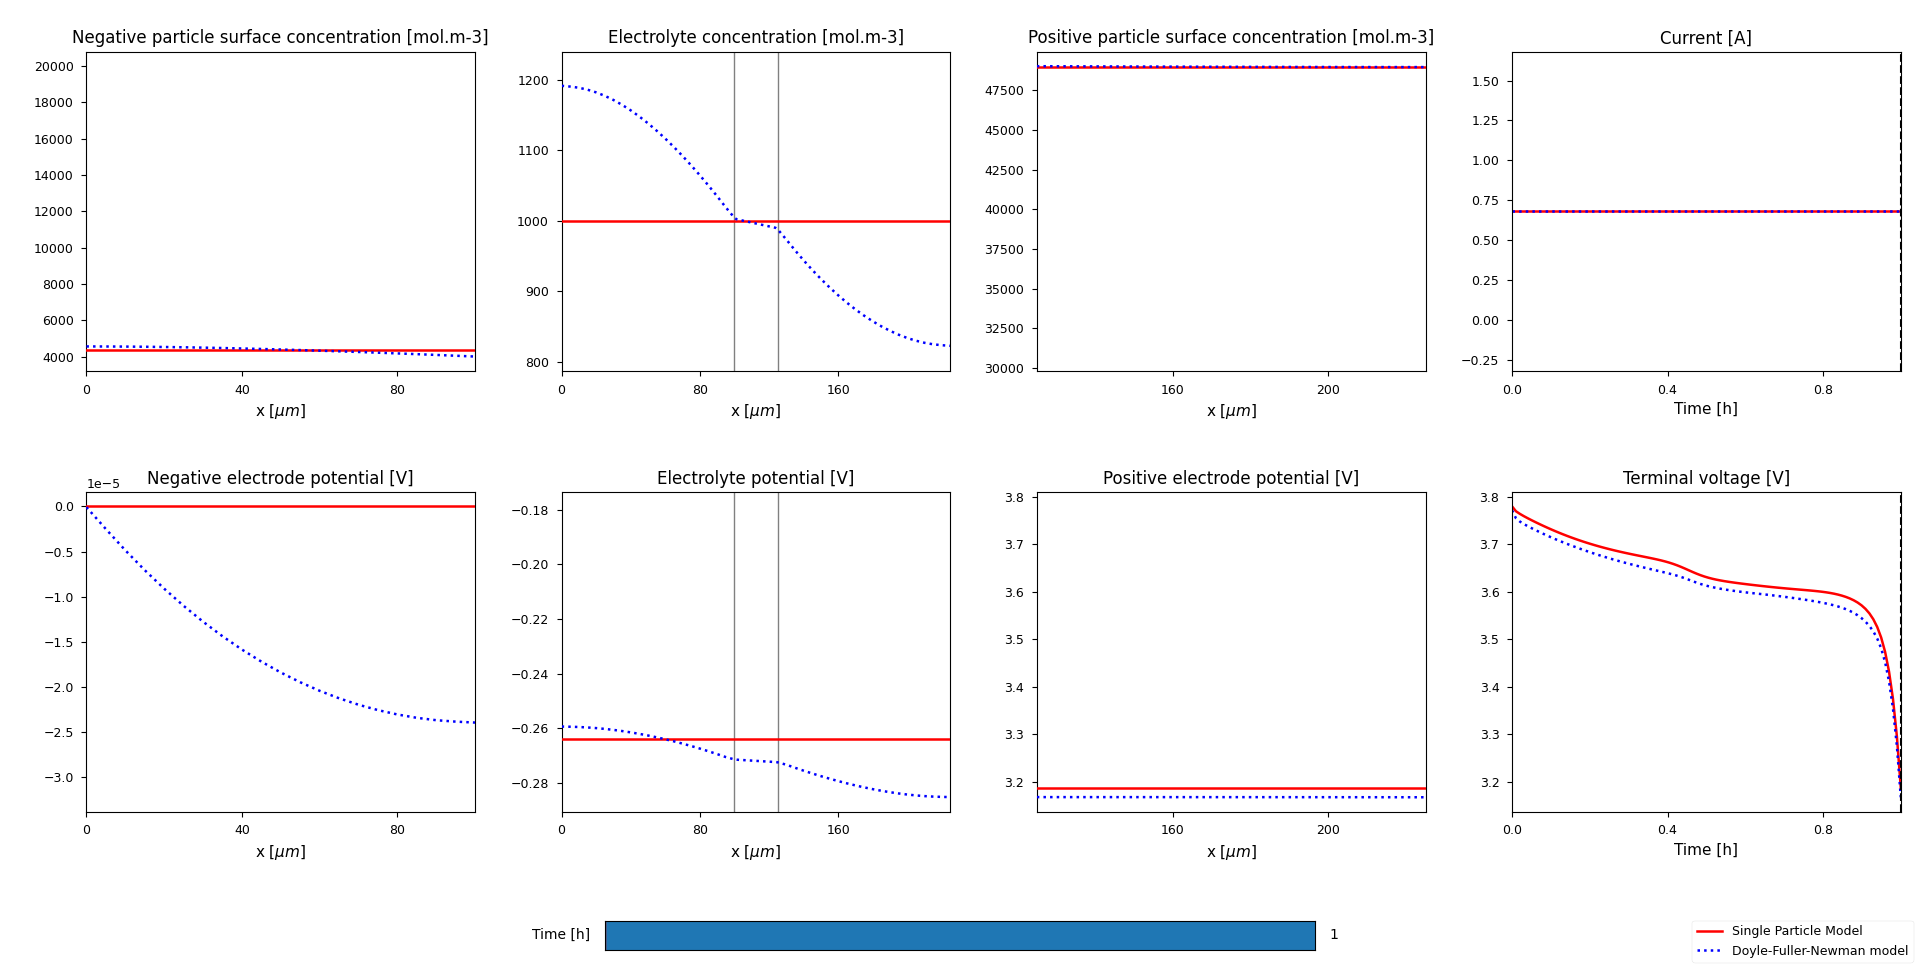
\includegraphics[scale = 0.32]{SPM-DFN3}
	\caption{单颗粒模型和DFN模型放电一小时对比图}
	\label{q}
\end{figure}

DFN图像结果解释(单颗粒模型见上):

negative particle surface concentration(负粒子溶度):
放电时,随着时间的变化,负极锂离子溶度下降。由于DFN模型需要考虑液相扩散,故需要关注电解质中的锂离子浓度,随着锂离子从负极固体颗粒中扩散经电解质溶液至正极固体颗粒,电解质中的锂离子先到达正极,故电解质中的锂离子浓度下降,低于负极锂离子浓度,因为二者的浓度差,故负极锂离子向电解质中扩散,于是二者浓度都下降,并且保持负极锂离子浓度高于电解质浓度,直至电解液浓度再次与负极锂离子浓度保持相同。于是有图中第一幅所表现的一样。

positive particle surface concentration(正粒子溶度):
放电时,随着时间的变化,正极锂离子浓度上升。锂离子从负极固体颗粒通过扩散经电解质溶液至正极固体颗粒。起始时,电解质中锂离子浓度与正极锂离子浓度保持大致相同,但通过负极锂离子的扩散,正极电解质中的锂离子浓度升高,并且高于正极锂离子浓度。基于正极处的电势较高,故电解质中的锂离子向正极扩散直至电解质锂离子浓度与正极锂离子浓度相等。于是有图中第三幅图所表现的一样。

Electrolyte concentration(电解质溶度):
在放电过程中,电解质中锂离子溶度相相同的,但是随着固相扩散和液相扩散的进行,负极锂离子向电解质中扩散,负极周围的电解质的锂离子浓度就有所升高,锂离子通过隔膜向正极周围电解质扩散,有快速向正极扩散,故正极周围的电解质锂离子浓度下降。直至放电结束,由于正极电势要高于负极电势,故正极周围电解质锂离子浓度高于负极锂离子浓度,且电势越高的地方,锂离子浓度相对较低,保持相对平衡,如图中第二幅图所表现的一样。

current(电流):
因为DFN同样采用的恒定电流测试,故电流不会发生改变。

negative electrode potential(负电极电位):
随着固相扩散的进行,有不断的电子产生又被转移至正极,故负极电势处于一个小波动变化的状态,但随着电子的全部转移,负极电势保持一个稳定的值。

positive electrolyte potential(正电极电位):
随着单颗粒锂离子电池模型中电子从负电极电位转移到正电极电位转移,正极锂离子与电子发生反应,从正极固体颗粒表面进入颗粒内部,故正极电势会逐渐下降。

electrolyte potential(电解质电位):
放电时,随着正极电势的下降,电解质中锂离子的扩散,电解质中的电势也就有所降低。

terminal voltage(电压):
随着正极固相扩散的进行,电子和锂离子发生反应,进入固体颗粒内部。导致正极电势的下降,故终端电压也逐渐减小。

\noindent\textbf{SPM与DFN图像结果比较解释}

negative particle surface concentration(负粒子溶度):
放电时,随着时间的变化,负极锂离子溶度下降。由于DFN模型需要考虑液相扩散,SPM模型不需要考虑液相扩散,故如图所示,在放电过程中,SPM模型的负极锂离子溶度与电解质锂离子溶度保持大致相同,DFM模型的负极锂离子溶度要略高于电解质锂离子浓度。两种模型的负极锂离子浓度与电解质浓度的起始和终止都保持相同。

positive particle surface concentration(正粒子溶度):
放电时,随着时间的变化,正极锂离子浓度上升。同样由于DFN考虑到液相扩散和电解质电势的变化过程,而SPM模型忽略了这些过程。故如图所示,在放电过程中,SPM模型的正极锂离子溶度与电解质锂离子溶度保持大致相同,DFN模型的正极锂离子溶度要略低于电解质锂离子浓度。两种模型的负极锂离子浓度与电解质浓度的起始和终止都保持相同。


Electrolyte concentration(电解质溶度):
在放电过程中,SPM模型的假设条件就是电解质中锂离子浓度保持不变,故电解质的锂离子溶度是不发生变化的,但DFN模型没有该种前提假设,故电解质浓度发生较大的变化,变化情况如图所示。

current(电流):
因为SPM和DFN同样采用的恒定电流测试,故电流不会发生改变。

negative electrode potential(负电极电位):
SPM假设正极负极和电解质内部电势都保持恒定不变,故在整个放电过程中,不会随着x的变化而变化,随着扩散现象的进行,忽略负极电子的产生和转移的动态过程,于是电势始终保持为0。DFN没有SPM的该种假设条件,故在放电过程中,电势都在在动态变化的,但是变化的大致趋向相同,DFN负极电势有所下降。

positive electrolyte potential(正电极电位):
无论SPM或DFN模型,由于正极一直在进行固相扩散现象,故电势的动态变化为平稳下降。

electrolyte potential(电解质电位):
SPM假设正极负极和电解质内部电势都保持恒定不变,故在整个放电过程中,不会随着x的变化而变化,随着扩散现象的进行,保持电解质内部电势相同,因为正极固相扩散的发生,总体趋势为下降。DFN没有SPM的该种假设条件,故在放电过程中,电势都在在动态变化的,但是变化的大致趋向相同,DFN电解质电势有所下降。

terminal voltage(电压):
随着正极固相扩散的进行,电子和锂离子发生反应,进入固体颗粒内部。导致正极电势的下降,故终端电压也逐渐减小。

\subsection{5 DFN电池模型对电池状态的估计}
可充电锂离子电池因其高能量、高功率密度、低放电率、低成本等优点,成为构建电网级储能系统的理想选择。对电池电池的老化成本进行精确建模是储能规划和运行的一个重要方面,尤其是在不规律的循环运行中。本文提出了一种半经验的锂离子电池退化模型,该模型从操作剖面评估电池寿命损失。我们通过结合电池退化的基本理论和我们的观察建立了这个模型。

电池退化模型可分为理论模型和经验模型。\cite{VETTER2005269}\cite{Ning_2004}\cite{NING20062012}的理论降解研究通常集中在锂离子等活性物质的损失方面。这些模型提供了各种退化机制的详细解释,以及它们是如何受到电池使用和条件的影响。然而,在规划阶段,人们只能预测BES的运行模式,没有关于详细的单元条件的信息。将操作水平的观察与分子水平的降解过程联系起来的理论研究仍然不足\cite{smith2014models}\cite{laresgoiti2015modeling}。因此,很难将充电和放电模式与发生在电池内部的分子水平过程直接联系起来。因此,要获得一个准确的电池退化经验模型,就需要对每个新应用进行特定操作的电池老化实验。这种测试需要几个月甚至几年的时间,并且必须在使用前进行。

电池的降解速率不仅取决于充电、放电、时间、温度等外部应力因素,还与电池当前的寿命状态有关。因此,电池退化是一个与时间和应力循环有关的非线性过程,这使得测试结果的分析和老化过程的预测建模复杂化。因此,我们提出了一个结合非线性分量和线性分量的退化模型。非线性成分模拟了SEI薄膜的形成过程,从而分析了电池寿命对降解的影响。分离这一效应可以建立不同应力因素的线性模型。

\noindent\textbf{1.日历和循环老化}

电池老化分为日历老化和循环老化\cite{VETTER2005269}\cite{laresgoiti2015modeling}\cite{wang2011cycle}\cite{millner2010modeling}\cite{kassem2012calendar}。日历老化反映了随着时间的推移,电池固有的退化,其速率受温度和电池SoC的影响。因此,在一段时间t上的日历老化$L_cal$可以表示为平均$SoC(\hat{\sigma})$和电池温度($\hat{T}_c)$的函数:
$$L_{cal} = f_t(t,\hat{\sigma},\hat{T}_c)$$

循环老化是指电池在每次充电和放电之间循环时所损失的寿命。我们用放电深度($\delta _i$)和循环平均SoC($\sigma_i$)来描述第i个循环。和平均粒子温度$T_{c,i}$. 由于我们将每个周期都建模为独立于其他周期的单个应力事件,累积的退化量是每个周期造成的容量减少量的总和。循环老化$L_{cyc}$则表示为:
$$L_{cyc} = \sum_{i}^{N}n_if_c(\delta _i,\sigma_i,\hat{T}_{c,i})$$
式中,N为操作中识别的周期数,$n_i$表示周期i是全周期还是半周期,用于融入循环计数算法。日历老化和周期老化是周期数的线性退化过程:
$$f_d(t,\delta,\sigma,T_c) = f_t(t,\hat{\sigma},\hat{T}_c) + \sum_{i}^{N}n_if_c(\delta_i,\sigma_i,T_{c,i})$$
当电池未运行时,N=0,仅为日历老化。我们可以将$f_d$写成一个关于单位时间内发生的退化的函数:
$$f_d = tf_t(t,\hat{\sigma},\hat{T}_c)$$

当电池运行由相同DoD和平均SoC的重复周期组成时,我们将日历和周期老化模型合并:
$$f_d^{cyc}(t,\delta,\sigma,T_c,N) = N(f_t(t_c,\sigma,T_c) + f_c(\delta,\sigma,T_c))$$
式中$t_c$为一个周期的持续时间。请注意,当所有循环相同时,单个循环的平均温度和SoC与整个操作的平均温度和SoC相同,因此$\hat{T} = T_c$和$\hat{\sigma} = \sigma$,$f_t$和$f_c$的温度和SoC输入是相同的。

提出的日历和周期老化模型表明,只要周期相同,降解率是相同的。然而,这不是我们在锂离子电池降解实验中观察到的。锂离子电池的降解速率对于循环次数并不是一个线性的过程,电池老化试验(图\ref{z})表明,在循环试验中,早期循环的降解速率明显高于后期循环,并在寿命结束(EoL)时迅速增加。

\begin{figure}[h]
	\centering
	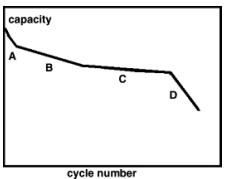
\includegraphics[scale = 0.7]{3}
	\caption{锂离子电池的一般容量退化行为}
	\label{z}
\end{figure}

这表明锂离子电池的降解速率取决于其当前的寿命状态。我们将电池寿命(L)纳入模型,并将实际的每循环降解率($dL/d(Cycle)$)表示为$f_L^{cyc}$的函数L和一个周期内的线性降解速率$f_d^{cyc}$
$$\frac{\partial L}{\partial(Cycle)} = f_L^{cyc}(L,f_d^{cyc})$$

其中L归一化为0到1,L = 0表示有新电池。电池寿命通常定义为电池仅提供其额定最大容量的80\%,即L = 0.2。

\noindent\textbf{2.SOC压力模型}

从下式得出SOC应力模型
$$S_\sigma = e^{k_\sigma(\sigma - \sigma_{ref})}$$
$k_\sigma$为SOC的应力系数,$\sigma_{ref}$为SOC水平的参考值,通常选择在0.4 ~ 0.5左右。来确定$k_\sigma$值,为不同日历老化试验数据SoC水平和测定$k_T$的类似方法可以使用。由试验数据可得$S_\sigma(\sigma_A)$如下:
$$S_{\sigma}(\sigma_A) = \frac{f_{d,t}[\sigma=\sigma_A]}{f_{d,t}[\sigma=\sigma_{ref}]}$$
该应力模型表明,在较高的温度下,降解速率较高的SoC级别和较低速率在较低的SoC级别,匹配塔菲尔的关系。然而,低SoC并不会增加容量衰落率,直接增加阻抗增大,功率增大减弱\cite{VETTER2005269},\cite{AMINE2001684},因此低SoC水平将加速循环老龄率。这项工作没有模拟这种效果,但应该会 与操作优化相结合。

\noindent\textbf{3.时间压力模型}

去除生活依赖和其他压力因素后,时间应力模型是时间的线性函数:
$$S_t(t) = k_tt$$
一旦温度和SoC应力模型系数($k_T$和$k_\sigma$),$k_t$可以很容易地计算出来,使用日历老化测试的结果: 
$$k_t = \frac{f_{d,t}[T=T_A,\sigma=\sigma_A]}{tS_T(T_A)S_{\sigma}(\sigma_A)}$$
式中$f_{d,t}[T=T_A,\sigma=\sigma_A]$表示线性化退化,在$T = T_A$,$\sigma = \sigma_a$的条件下,T为日历老化测试的持续时间。

在指定的环境条件和运行模式下,大多数电池退化测试结果记录电池容量与周期数(循环老化测试)的关系(图\ref{y})。

\begin{figure}[H]
	\centering
	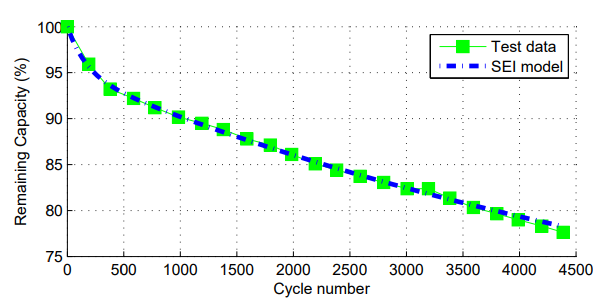
\includegraphics[scale = 0.6]{4}
	\caption{退化曲线和SEI模型的拟合实例}
	\label{y}
\end{figure}

对DFN模型进行评估,计算锂电池可重复充电次数,寿命。如图\ref{y},可进行仿真进行估计,考虑从初始100\%的电池容量到达整体容量的80\%的过程,可重复的循环次数大约是3600次深度充放电过程。
\section{模型评价}
SPM模型优点:对于问题一和问题二,主要应用了SPM模型,它是最简单的锂离子电池电化学模型,是简化了DFN模型简化而来的。通过简化锂离子电池的工作状态,将电池的正负极看成单个球形颗粒,SPM的无量纲形式在每个电极中只解一个粒子的扩散方程,而不是像DFN模型那样在每个宏观点上解一个粒子的扩散方程。这个模型不应被解释为用单个粒子取代电极中的许多粒子。相反,在这个极限下,电极中的所有粒子都以完全相同的方式行为,因此只解一个代表粒子就足够了。省略液相扩散过程,使电解质的锂离子浓度保持不变。省略液相电势过程,使电池内部电势保持不变。通过简化的单粒子模型结构简单,运算量小,容易实现在线应用和实验数据估计。模型的模拟速度能够大大提升,所需要的时间大大减少。

SPM模型缺点:锂离子电池单粒子模型存在一些不可避免的缺点,如在大倍率充放电条件下,模型的无液相扩散和无液相电势等假设是不可理的,因此导致仿真偏差过大,模型测试的实验结果数据偏离锂离子电池的真实工作状态,会对电池荷电状态、电池健康状况和电池寿命等判断产生重大偏差。

DFN模型优点:DFN模型又被称为准二维(P2D)模型或Newman模型,该模型由一组高度耦合的非线性抛物线型和椭圆型偏微分方程组成,该方程可以由多个不同的数值方法求解,包括有限差分法、控制体积、有限元法和正交配置等。以隐式假定电流在某一点等于电极平均电流,这就意味着DFN模型的每个粒子的浓度在所有操作条件下都是相同的,这在低电流的情况下是更有效的。使用复杂的数值技术,DFN模型对于某些应用来说,在计算上虽然过于复杂。例如电池管理系统采用等效电路模型,它只包含少量的常微分方程。但是相对于SPM模型,DFN模型所得到的数值精确度更高,通过DFN模型进行电池模拟更加贴合实际场景。DFN模型更适合于实验室研究,用于辅助分析电池的衰减老化机制及诊断其状态,以及通过仿真模拟锂离子电池的优化设计(修改材料颗粒设计、扩散系数调整方向等)进行理论支持。

DFN模型缺点:
锂离子电池DFN模型过于复杂,计算量大,且无法获得其解析解,即使使用复杂的数值技术,DFN模型对于某些应用来说在计算上仍然过于复杂,对硬件要求高,如运行速度、内存要求及数值收敛等要求更高。 

改进:模型的设计可考虑了电池的几个基本理论,包括阿伦尼乌斯关系和SEI膜的形成。本文推导的参数来源于特定类型锂离子电池的仿真实验数据,而所提出的模型和参数整定方法无法应用于其他类型锂离子电池的模型。
\newpage
\bibliographystyle{cjc}
\bibliography{example}
\newpage
\begin{center}
	\large{\textbf{附\quad 录}}
\end{center}
\begin{Python}{SPM锂离子电池模拟实验1}
import pybamm
import numpy as np
import matplotlib.pyplot as plt

model = pybamm.lithium_ion.SPM()
geometry = model.default_geometry

param = model.default_parameter_values
param.process_model(model)
param.process_geometry(geometry)
mesh = pybamm.Mesh(geometry, model.default_submesh_types, model.default_var_pts)
disc = pybamm.Discretisation(mesh, model.default_spatial_methods)
disc.process_model(model);



solver = model.default_solver
n = 250
t_eval = np.linspace(0, 3600, n)
print('Solving using',type(solver).__name__,'solver...')
solution = solver.solve(model, t_eval)
print('Finished.')

voltage = solution['Terminal voltage [V]']
current = solution['Current [A]']
Lithium_concentration = solution['Electrolyte concentration [mol.m-3]']
c_s_n_surf = solution['Negative particle surface concentration']
c_s_p_surf = solution['Positive particle surface concentration']
a = solution['Electrolyte potential [V]']

t = solution["Time [s]"].entries
x = solution["x [m]"].entries[:, 0]
f, (ax1, ax2, ax3, ax4, ax5, ax6) = plt.subplots(1, 6, figsize=(13,6))

ax1.plot(t, voltage(t))
ax1.set_xlabel(r'$Time [s]$')
ax1.set_ylabel('Terminal voltage [V]')

ax2.plot(t, c_s_n_surf(t=t, x=x[0]))  # can evaluate at arbitrary x (single representative particle)
ax2.set_xlabel(r'$Time [s]$')
ax2.set_ylabel('Negative particle surface concentration')

ax3.plot(t, c_s_p_surf(t=t, x=x[-1]))  # can evaluate at arbitrary x (single representative particle)
ax3.set_xlabel(r'$Time [s]$')
ax3.set_ylabel('Positive particle surface concentration')

ax4.plot(t, current(t))  # can evaluate at arbitrary x (single representative particle)
ax4.set_xlabel(r'$Time [s]$')
ax4.set_ylabel('Current[A]')

ax5.plot(t, Lithium_concentration(t=t, x=x[-1]))  # can evaluate at arbitrary x (single representative particle)
ax5.set_xlabel(r'$Time [s]$')
ax5.set_ylabel('Electrolyte concentration [mol.m-3]')

ax6.plot(t, Lithium_concentration(t=t, x=x[-1]))  # can evaluate at arbitrary x (single representative particle)
ax6.set_xlabel(r'$Time [s]$')
ax6.set_ylabel('Electrolyte potential [V]')

plt.tight_layout()
plt.show()
\end{Python}
\begin{Python}{SPM锂离子电池模拟实验2}
	import pybamm
	
	pybamm.set_logging_level("INFO")
	
	# load models
	model = pybamm.lithium_ion.SPM(),
	
	# create and run simulations
	sims = []
	
	sim = pybamm.Simulation(model)
	sim.solve([0, 3600])
	sims.append(sim)
	
	# plot
	pybamm.dynamic_plot(sims)
\end{Python}
\begin{Python}{比较单颗粒模型不同温度模型}
	import pybamm
	
	options1 = {"thermal": "isothermal"}
	options2 = {"thermal": "lumped"}
	options3 = {"thermal": "x-lumped"}
	options4 = {"thermal": "x-full"}
	
	models = [pybamm.lithium_ion.SPM(options=options1, name= "isothermal"),
	pybamm.lithium_ion.SPM(options=options2, name= "lumped"),
	pybamm.lithium_ion.SPM(options=options3, name= "x-lumped"),
	pybamm.lithium_ion.SPM(options=options4,name ="x-full"),
	]
	solutions = ["isothermal", "lumped", "x-lumped", "x-full"]
	
	for i, model in enumerate(models):
	sim = pybamm.Simulation(model)
	sim.solve([0, 3700])
	solutions[i] = sim.solution
	
	
	plot = pybamm.QuickPlot(solutions)
	plot.dynamic_plot()
\end{Python}
\begin{Python}{比较单颗粒模型不同扩散模型}
import pybamm

models = [
	pybamm.lithium_ion.SPM(
	options={"particle": "Fickian diffusion"}, name="Fickian diffusion"   # 菲克扩散
	),
	pybamm.lithium_ion.SPM(
	options={"particle": "uniform profile"}, name="uniform profile"       # 统一轮廓,均匀分布
	),
	pybamm.lithium_ion.SPM(
	options={"particle": "quadratic profile"}, name="quadratic profile"    # 二次曲线,二次分布
	),
	pybamm.lithium_ion.SPM(
	options={"particle": "quartic profile"}, name="quartic profile"       # 四次轮廓,四次分布
	),
]

experiment = pybamm.Experiment(
	["Discharge at C/10 for 10 hours or until 3.3 V",
	"Rest for 1 hour",
	"Charge at 1 A until 4.1 V",
	"Hold at 4.1 V until 50 mA",
	"Rest for 1 hour",]
)

sims = []
for model in models:
	sim = pybamm.Simulation(model, experiment=experiment)
	sim.solve([0, 3600])
	sims.append(sim)
	print("Particle model: {}".format(model.name))
	print("Solve time: {}s".format(sim.solution.solve_time))

pybamm.dynamic_plot(sims)
\end{Python}
\begin{Python}{两者模型比较}
import pybamm

pybamm.set_logging_level("INFO")


models = [
	pybamm.lithium_ion.SPM(),
	pybamm.lithium_ion.DFN(),
]


sims = []
for model in models:
	sim = pybamm.Simulation(model)
	sim.solve([0, 3600])
	sims.append(sim)

pybamm.dynamic_plot(sims)
\end{Python}


\end{document}